\documentclass{article}
% to compile a camera-ready version, add the [final] option, e.g.:
    \usepackage[final]{neurips_2019}

\usepackage[utf8]{inputenc} % allow utf-8 input
\usepackage[T1]{fontenc}    % use 8-bit T1 fonts
\usepackage{hyperref}       % hyperlinks
\usepackage{url}            % simple URL typesetting
\usepackage{booktabs}       % professional-quality tables
\usepackage{amsfonts}       % blackboard math symbols
\usepackage{nicefrac}       % compact symbols for 1/2, etc.
\usepackage{microtype}      % microtypography
\usepackage{amsmath}

\usepackage{graphicx}
\usepackage{mathdots}
\usepackage[english]{babel}
\usepackage[justification=centering]{caption}
\usepackage{placeins}

\usepackage{times}
\usepackage{array}
\usepackage{mathtools}
\usepackage{float}
\usepackage[ruled,vlined]{algorithm2e}
\usepackage{natbib}

\newcommand{\bunderline}[1]{\underline{#1}}
\renewcommand{\vec}[1]{{\bunderline{#1}}}
\newcommand{\vect}[1]{{\bunderline{#1}}} 
\newcommand{\mat}[1]{{\bunderline{\bunderline{#1}}}}

\title{Solving the Radiative Transfer Equations via the Radon Transform}

\author{%
  Eappen Nelluvelil \\
  Rice University \\
  \texttt{esn2@rice.edu} \\
  \And
  Megan Oeltjenbruns \\
  Wayne State College \\
  \texttt{meoelt01@wsc.edu} \\
  \And
  Jacob Spainhour \\
  Florida State University \\
  \texttt{jcs15c@my.fsu.edu} \\
}

\begin{document}

\maketitle

\begin{abstract}

We aim to efficiently solve multi-dimensional partial differential equations using the Radon transform. By applying the Radon transform to such a 2D PDE, we reduce the problem to a collection of 1D PDEs that can be time-stepped up to a desired final time. Following this, the inverse of the Radon transform is applied to return the new solution to physical space. We specifically apply this method to the $P_N$ approximation for radiative transfer, a hyperbolic system of linear PDEs.

\end{abstract}

% !TEX root = main.tex

%%%%%%%%%%%%%%%%%%%%%%%%%%%%%%%%%%%%%%%%%%%%%%%%%%%%%%%%%%%%%%%%%%
\section{Introduction}

%%%%%%%%%%%%%%%%%%%%%%%%%%%%%%%%%%%%%%%%%%%%%%%%%%%%%%%%%%%%%%%%%%
\subsection{Imaging}

The Radon transformation commonly seen alongside imaging problems.
Fundamentally, the imaging problem attempts to reconstruct a distribution from measurements taken at several different angles.
A familiar example of this is any kind of medical imaging device, such as an MRI machine.
The device collects measurements from several angles, which are used to reconstructed an accurate image.
When applied to a mathematical function, the Radon transform produces these measurements, or more accurately profiles, with integrals.
Likewise, the inverse Radon transform restores the original function from a collection of profiles spanning all angles.
Many properties of the Radon transform cause standard PDE solution methods to be simpler on the profiles than on the original domain.
For this paper specifically, we take advantage of the dimension-intertwining properties of the Radon transform to simplify solution methods of hyperbolic PDEs.

%%%%%%%%%%%%%%%%%%%%%%%%%%%%%%%%%%%%%%%%%%%%%%%%%%%%%%%%%%%%%%%%%%
\subsection{Previous Work}

Existing literature regarding this method is sparse.
Much of the theoretical groundwork is owed to the work of \textit{Dimensional Splitting of Hyperbolic Partial Differential Equations using the Radon Transform} by Donsub Rim.\cite{Rim:5}
Here, Rim was able to use a coarse approximation to the Radon transform to use large time stepping methods to solve the hyperbolic PDEs we are interested in.
Our method follows the same basic procedure, but uses a more accurate forward and inverse Radon transform to produce more numerically viable results.
% !TEX root = main.tex

%%%%%%%%%%%%%%%%%%%%%%%%%%%%%%%%%%%%%%%%%%%%%%%%%%%%%%%%%%%%%%%%%%
\section{The Radon Transform and Backprojection}

%%%%%%%%%%%%%%%%%%%%%%%%%%%%%%%%%%%%%%%%%%%%%%%%%%%%%%%%%%%%%%%%%%
\subsection{The Radon Transform}

To properly introduce the Radon transform, we begin with the standard $xy$ coordinate system on which our solution lies.
If we rotate our axes by a positive angle $\omega$ with respect to the positive $x$-axis, we obtain a new $sz$ coordinate system.
\par 
Given a point $\left( s, z \right)$ in this $sz$ coordinate system, we can write the same point in the $xy$ coordinate system using a rotation matrix:
\begin{align*}
    \begin{bmatrix}
        x \\
        y
    \end{bmatrix}
    & = 
    \begin{bmatrix}
        \cos (\omega) & -\sin (\omega) \\
        \sin (\omega) & \cos (\omega)
    \end{bmatrix}
    \begin{bmatrix}
        s \\
        z
    \end{bmatrix}
\end{align*}
Likewise, given a point $\left( x, y \right)$ in the $xy$ coordinate system, we can rewrite it in the $sz$ coordinate system using the inverse of the rotation matrix:
\begin{align*}
    \begin{bmatrix}
        s \\
        z
    \end{bmatrix}
    & = 
    \begin{bmatrix}
        \cos (\omega) & \sin (\omega) \\
         -\sin (\omega) & \cos (\omega)
    \end{bmatrix}
    \begin{bmatrix}
        x \\
        y
    \end{bmatrix}
\end{align*}
% We introduce the Radon transform using this change of coordinate formulas.
% \begin{align*}
%     x \left( s, z; \omega \right) & = s\, \cos \left( \omega \right) - z\,\sin \left( \omega \right) \\
%     y \left( s, z; \omega \right) & = s\, \sin \left( \omega \right) + z\,\cos \left( \omega \right) \\
%     s \left( x, y; \omega \right) & = x \cos \left( \omega \right) + y \sin \left( \omega \right) \\
%     z \left( x, y; \omega \right) & = -x \sin \left( \omega \right) + y \cos \left( \omega \right)
% \end{align*}
Suppose $f(x, y): \mathbb{R}^{2} \rightarrow \mathbb{R}$ is a function with compact support. 
The \textbf{Radon transform} of $f$, denoted $\mathcal{R} \left( f \right) (s, \omega) = \widehat{f}(s, \omega)$, is defined as follows:
\begin{align*}
    \mathcal{R}(f) \left( s, \omega \right) & := \int_{-\infty}^{\infty} f \left(s \cos \left( \omega \right) - z \sin \left( \omega \right), s \sin \left( \omega \right) + z \cos \left( \omega \right) \right) \, dz
\end{align*}
Geometrically, the Radon transform fixes an angle $\omega$, generates a rotated $sz$ axis, then integrates $f$ along $s$ parallel to the $z$ axis.\cite{Press:4}.
When we are interested in the Radon transform of a specific point, we compute a single line integral.
\subsection{Intertwining Property of the Radon Transform}
The property of the Radon transform we will most explot is its effect on spatial partial derivatives.
Specifically, spatial derivatives in $x$ and $y$ become intertwined, transforming into partial derivatives in $s$.
By the chain rule, we obtain the following formulas for partial derivatives with respect to $x$ and $y$:
\begin{align*}
	\frac{\partial}{\partial x} & = \frac{\partial s}{\partial x} \frac{\partial}{\partial s} + \frac{\partial z}{\partial x} \frac{\partial}{\partial z} \\
	\frac{\partial}{\partial y} & = \frac{\partial s}{\partial y} \frac{\partial}{\partial s} + \frac{\partial z}{\partial y} \frac{\partial}{\partial z}
\end{align*}
We recall definitions for coordinate transform, and can use them to compute derivatives directly.
\begin{align*}
    \frac{\partial s}{\partial x} & = \cos \left( \omega \right) & \frac{\partial z}{\partial x} & = -\sin \left( \omega \right) \\
    \frac{\partial s}{\partial y} & = \sin \left( \omega \right) & \frac{\partial z}{ \partial y} & = \cos \left( \omega \right)
\end{align*}
Substituting these into our chain rule derived formula, we obtain the following:
\begin{align*}
	\frac{\partial}{\partial x} & = \cos \left( \omega \right) \frac{\partial}{\partial s} -\sin \left( \omega \right) \frac{\partial}{\partial z} \\
	\frac{\partial}{\partial y} & = \sin \left( \omega \right) \frac{\partial}{\partial s} + \cos \left( \omega \right) \frac{\partial}{\partial z}
\end{align*}
We now consider $\mathcal{R} \left( f_{,x} \right) \left( s, \omega \right)$.
\begin{align*}
    \mathcal{R} \left( f_{,x} \right) \left( s, \omega \right) & = \int_{-\infty}^{\infty} f_{, x} \, dz  \\
    & = \int_{-\infty}^{\infty}  \left( \cos (\omega) \, f_{, s} - \sin (\omega) \, f_{, z} \right) \, dz \\
    & = \cos (\omega) \int_{-\infty}^{\infty} f_{, s} \, dz - \sin (\omega) \int_{-\infty}^{\infty} f_{, z} \, dz \\
    & = \cos (\omega) \frac{\partial}{\partial s} \int_{-\infty}^{\infty} f\,dz - \sin (\omega) \left[\, f \left( z = +\infty \right) - f \left(z = -\infty \right) \right] \\
    & = \cos (\omega) \, \frac{\partial}{\partial s} \mathcal{R}(\,f) \left( s, \omega \right) \\
    & = \cos (\omega) \, \widehat{f}_{,s} \left( s, \omega \right)
\end{align*}
Likewise for $\mathcal{R} \left( f_{,y} \right) \left( s, \omega \right)$:
\begin{align*}
    \mathcal{R} \left( f_{,y} \right) \left( s, \omega \right) & = \int_{-\infty}^{\infty} f_{, y} \, dz  \\
    & = \int_{-\infty}^{\infty}  \left( \sin (\omega) \, f_{, s} - \cos (\omega) \, f_{, z} \right) \, dz \\
    & = \sin (\omega) \int_{-\infty}^{\infty} f_{, s} \, dz - \cos (\omega) \int_{-\infty}^{\infty} f_{, z} \, dz \\
    & = \sin (\omega) \frac{\partial}{\partial s} \int_{-\infty}^{\infty} f\,dz - \cos (\omega) \left[\, f(z = +\infty) - f(z = -\infty) \right] \\
    & = \sin (\omega) \, \frac{\partial}{\partial s} \mathcal{R}(\,f) \left( s, \omega \right) \\
    & = \sin (\omega) \, \widehat{f}_{,s} \left( s, \omega \right)
\end{align*}
In summary,
\begin{align*}
    \mathcal{R} \left( f_{,x} \right) \left( s, \omega \right) & = \cos (\omega) \, \widehat{f}_{,s} \left( s, \omega \right) \\
    \mathcal{R} \left( f_{,y} \right) \left( s, \omega \right) & = \sin (\omega) \, \widehat{f}_{,s} \left( s, \omega \right)
\end{align*}
We have successfully reduced our spatial derivatives to a single dimension.

%%%%%%%%%%%%%%%%%%%%%%%%%%%%%%%%%%%%%%%%%%%%%%%%%%%%%%%%%%%%%%%%%%
\subsection{Discretizing the Radon Transform}

To properly implement the Radon transform in our software, we begin by restricting our non-zero domain to be the unit circle, satisfying our compact support.
Within this circle, we must select points for a mesh, along which we compute the Radon transform.
As $\omega$ is constant across each profile of the Radon transform, we establish $N_\omega$ uniformly spaced diameters.

We also must consider the spacing of points along each diaeter.
Rather than uniformly spacing these points, as doing so would introduce Runge phenomena, Chebyshev points of the second kind are placed along each diameter.
These aregenerated according to the following formula:

\begin{align*}
    \cos\left(\frac{j\pi}{N_s}\right) \\
    j = 1, 2, \dots, N_s
\end{align*}

By using Chebyshev points, the interpolation and differentiation methods we later used are guaranteed to be accurate.
That is to say, for $C^\infty$ functions, the error of these methods rapidly converges to zero.

%%%%%%%%%%%%%%%%%%%%%%%%%%%%%%%%%%%%%%%%%%%%%%%%%%%%%%%%%%%%%%%%%%
\subsection{Quadrature and Interpolation}

Because we assume compact support on the unit circle, it is possible to determine the Radon transform at a point by computing the requisite line integral across a chord of the domain, whose length is denoted as $2\tau$, rather than to infinity.
The integration is then performed using the Clenshaw-Curtis quadrature.
The $N_q$ nodes used are Chebyshev points, with weights are derived through the fast Fourier transform.\cite{Trefethen:7} 
\begin{align*}
	\mathcal{R}(\,f) &= \int_{-\infty}^{\infty} f(x, y) \, dz = \int_{-\tau}^{\tau} f(x, y) \, dz \approx \sum_{i=1}^{N_q} w_{i} \, f(z_{i})
\end{align*}
Applied to our Radon transform, the formula is as follows:
\begin{align*}
    \mathcal{R}(\,f)(s, \omega) \approx \, & \tau \sum_{k=0}^{N_q} w_{k} \, f(s_{i} \cos (\omega_{j}) - \tau t_{k} \sin (\omega_{j}), \, s_{i} \sin (\omega_{j}) + \tau t_{k} \cos (\omega_{j}))
\end{align*}
where $t_k$ are Chebyshev points on the interval $[-1, 1]$.
% This process is implemented through the following psuedocode:

% \noindent\fbox{
%     \parbox{\textwidth}{
%         theta = \pi arange(0, N, 1) / (N-1)
%         x = \cos(\theta)
%         w = zeros((N,))
%         ii = arange(1, N-1)
%         v = ones((N-2,))
%         if (N-1) \% 2 == 0:
%         \quad w[0] = 1/((N-1)**2-1)
%         \quad w[N] = w[0]
%         \quad for k in range (1, (N-1)//2):
%         \quad \quad v = v - 2*\cos(2*k*\theta[ii])/(4*k**2-1)
%         \quad v = v - \cos(N*\theta[ii])/(N**2-1)
%         else:
%         \quad w[0] = 1/((N-1)**2)
%         \quad w[N] = w[0]
%         \quad for k in range (1, (N-2)//2 + 1):
%         \quad \quad v = v - 2*\cos(2*k*\theta[ii])/(4*k**2-1)
%         w[ii] = 2*v/(N-1)
%         return x, w}}

% \begin{algorithm}
%     \caption{Discretized Radon Transform}
%     \KwIn{$\vec{f} \in \mathbb{R}^{N_{s} \times N_{\omega}}$ \\
%     $N_{s}$, the number of discretization points along one angle \\
%     $N_{\omega}$, the number of angles \\
%     $N_{q}$, the number of quadrature points to use for line integrals}
%     \KwOut{$\vec{\widehat{f}} \in \mathbb{R}^{N_{s} \times N_{\omega}}$}
%     \hrulefill \\
%     \nl $s \gets$ \texttt{clen\_curt}()\;
% \end{algorithm}
    
\begin{figure}[H]
	\centering
	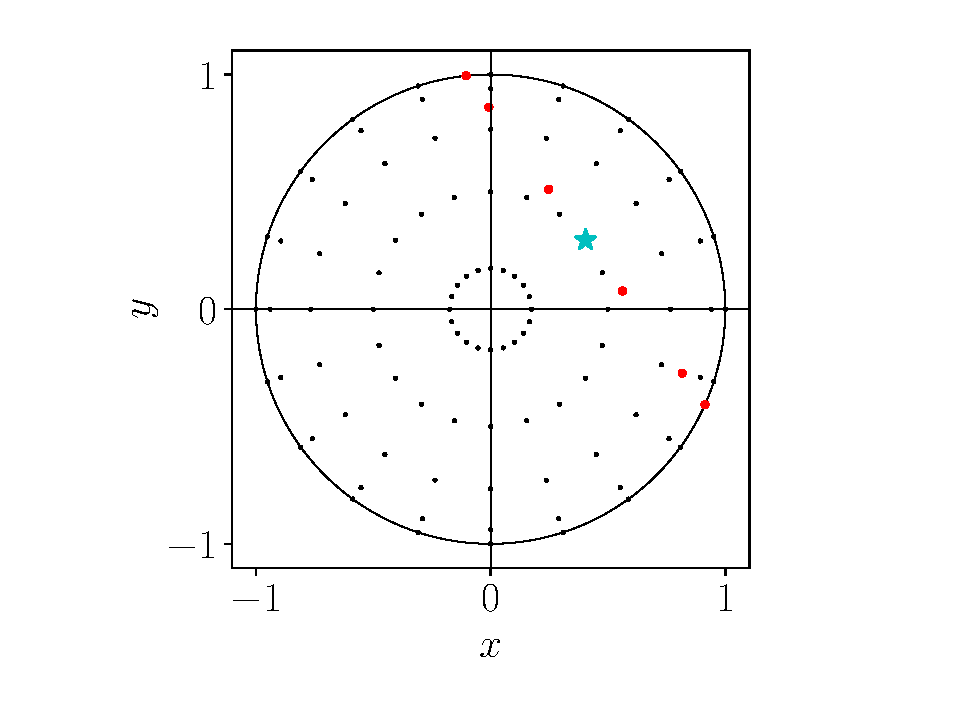
\includegraphics[scale=0.5]{figures/quad_5.pdf}
    \caption{6 point quadrature rule for the point $(x,y)$, denoted by a blue star.\\ Quadrature nodes labeled red, grid points labeled black}
\end{figure}
    
For the purposes of computing the proper inverse Radon transform, we perform the forward Radon transform as if we only know $f$ at the predefined grid points.
However, as shown in the figure above, these points rarely line up exactly with the points needed for quadrature.
Therefore, interpolation needs to be done to find those function values.
To obtain as much accuracy in the interpolation as possible, a series of one-dimensional interpolation schemes.
The point at which $f$ needs to be approximated is first projected onto the four closest diameters.
Barycentric interpolation is then performed along these diameters.
The stabilized barycentric interpolation formula \cite{Trefethen:7} is reproduced below.
\begin{align*}
    H_n(x)&= \frac{\sum_{j = 0}^{n} \alpha_j \frac{f_j}{x-x_j}}{\sum_{j = 0}^{n} \alpha_j\frac{1}{x-x_j}} \\ 
    \alpha_0 = \frac{1}{2},\quad \alpha_{1:n-1} = &(-1)^{1:n-1},\quad \alpha_n = \frac{1}{2} (-1)^n \\
\end{align*} 
Next, four point polynomial interpolation is performed across these four points.
Let $\theta_0$ be the midpoint of the arc containing $h_i$, $i=1,\dots,4$, obtained through barycentric interpolation:
\begin{align*}
    p(\theta) = - &\frac{1}{16}(h_1 - 9h_2 - 9h_3 + h_4) \\
    + &\frac{1}{24d\omega}(h_1 - 27h_2 + 27h_3 - h_4)(\theta - \theta_0) \\
    + &\frac{1}{4d\omega^2}(h_1 - h_2 - h_3 + h_4)(\theta - \theta_0)^2 \\
    - &\frac{1}{6d\omega^3}(h_1 - 3h_2 + 3h_3 - h_4)(\theta - \theta_0)^3
\end{align*}
\begin{figure}[H]
	\centering
	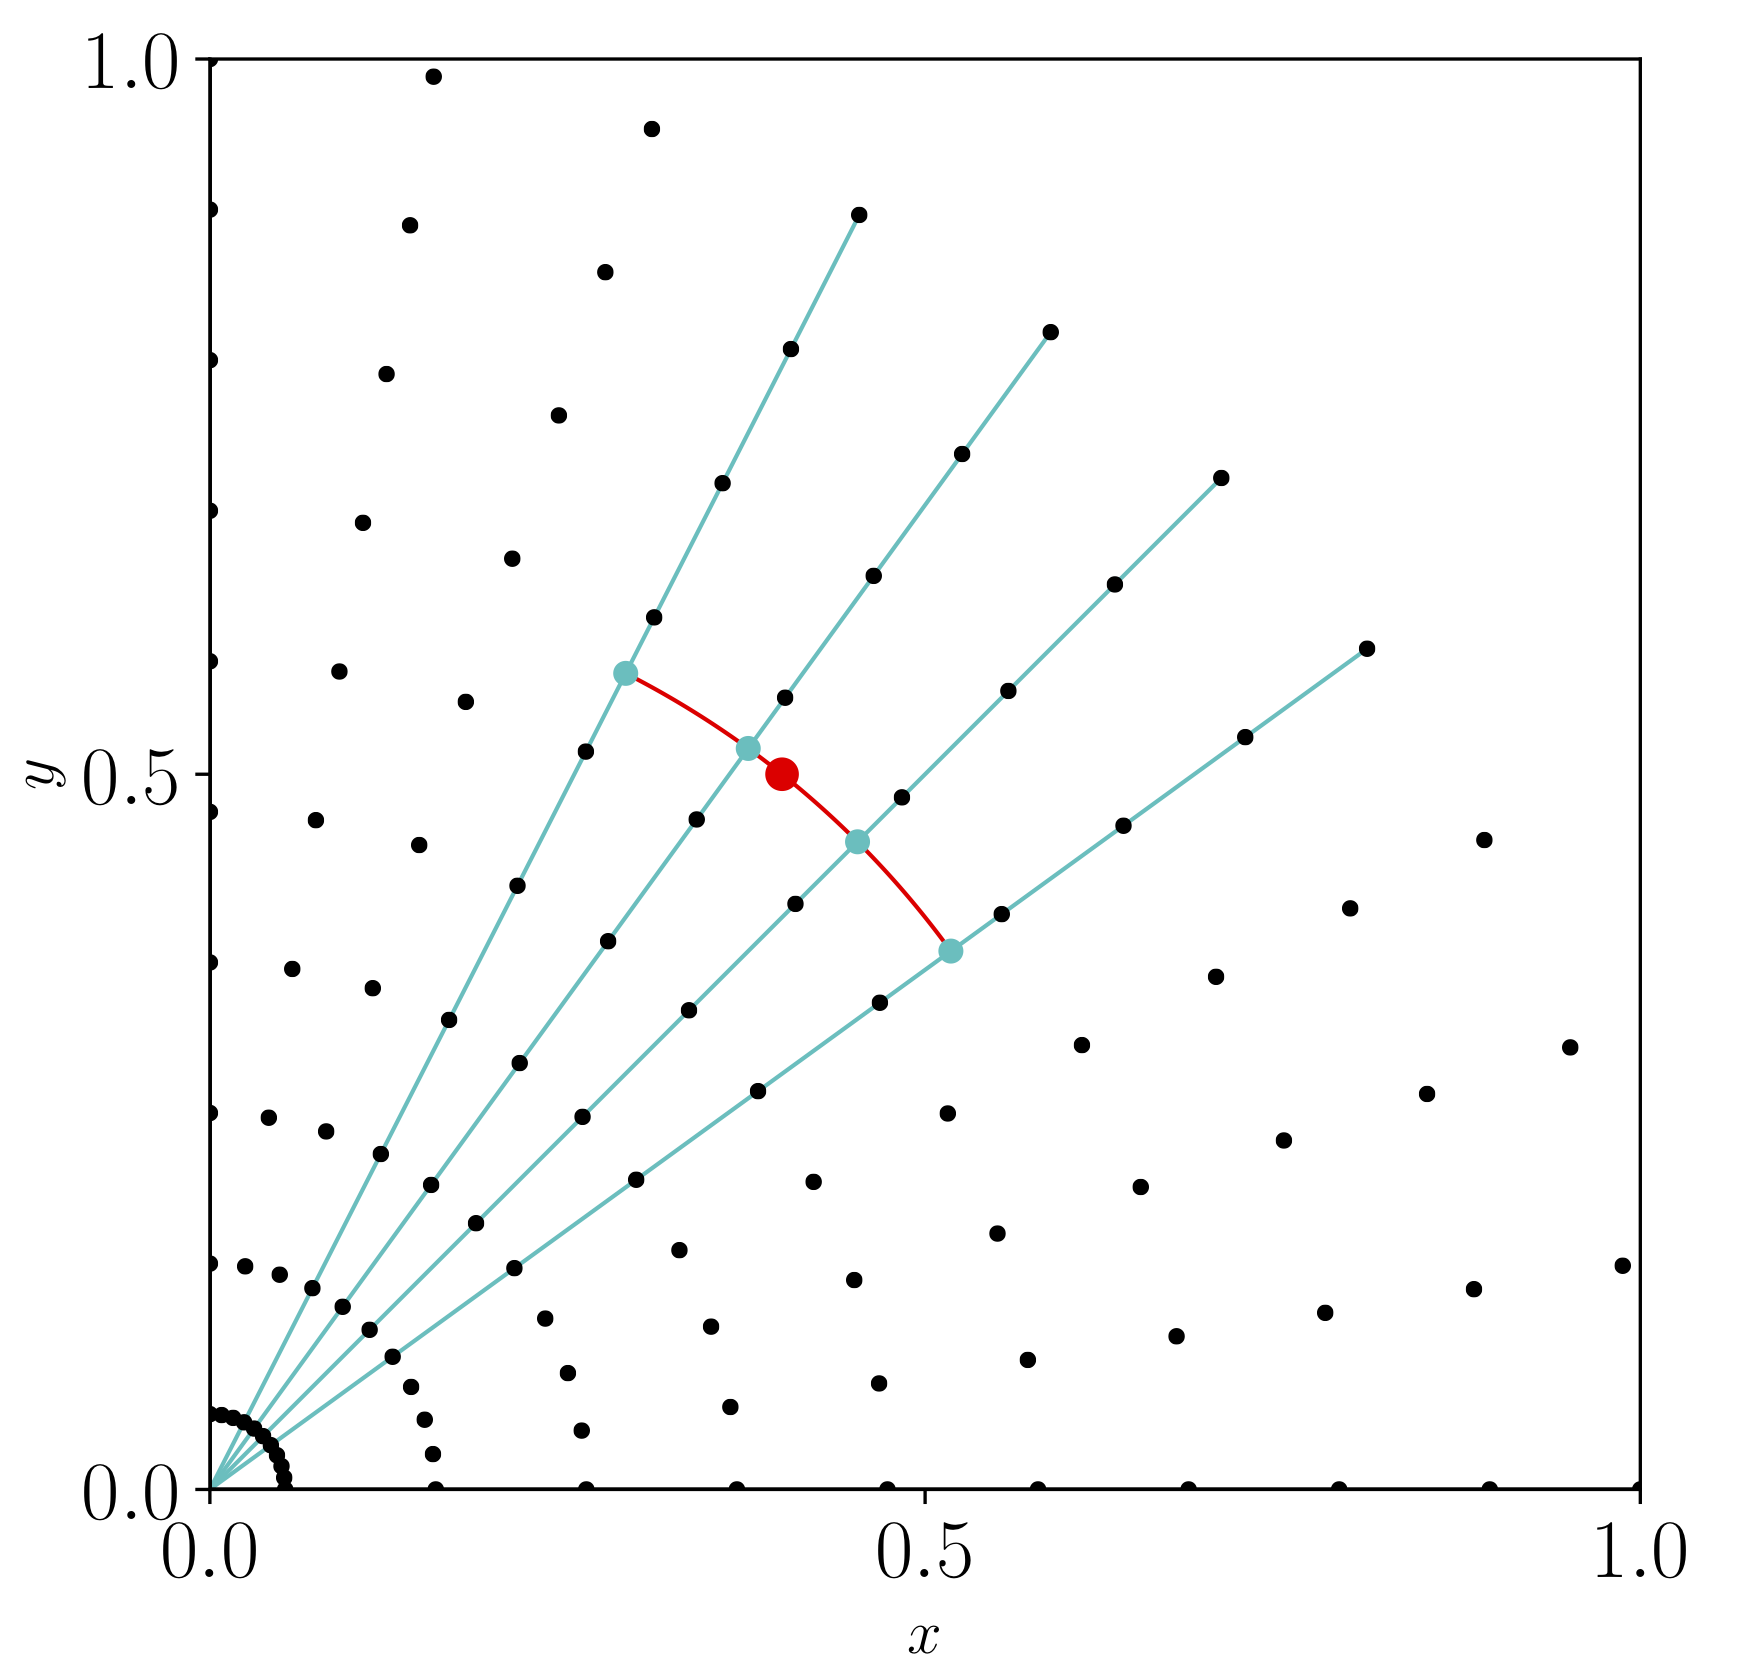
\includegraphics[scale=0.5]{figures/Interp4.png}
	\caption{Approximates $f$ at a point $(x, y)$, labeled with a red dot, \\using the values calculated at the four points labeled with a blue dot}
\end{figure}

This interpolation procedure is performed for each quadrature point for a single Radon transform evaluation.
The quadrature method itself is applied to each point in the grid, resulting in the Radon transform of our discretized domain.

\subsection{Backprojection}

The adjoint of the Radon transform, denoted $\mathcal{R}^{*}$, is known as \textbf{backprojection}. 
\par 
Given a function $\widehat{f}(s, \omega): \mathbb{R} \times \left[ 0, \pi \right] \rightarrow \mathbb{R}$, the backprojection of $\widehat{f}$ is defined as follows:
\begin{align*}
    \mathcal{R}^{*} \left( \widehat{f} \, \right) (x, y) := \int_{0}^{\pi} \widehat{f} \left( x \cos \left( \omega \right) + y \sin \left( \omega \right), \omega \right) \, d \omega
\end{align*}
Geometrically, the backprojection of $\widehat{f}$ at a point $\left( x, y \right)$ is the integral along the circle whose diameter is the line segment connecting $(x, y)$ and the origin.
\par 
The backprojection is useful in computing a stable inverse Radon transform \cite{Press:4}.

\subsection{Discretizing the Backprojection}

As was the case with the Radon transform, we need to discretize the backprojection for computational purposes.
Recall that our underlying mesh is parameterized by two integers:
\begin{itemize}
    \item $N_{\omega}$, the number of equi-spaced angles
    \item $N_{s}$, the number of Chebyshev points of the second kind along any one angle
\end{itemize}
This means our mesh consists of $N_{p} := N_{\omega} \times N_{s}$ points.
\par 
Given a function $\widehat{f} \left( s, \omega \right)$, we want to compute the \textit{approximate} backprojection $\widehat{f}$ at a mesh point $\left( x_{k}, y_{k} \right)$ where $k = 1, 2, \hdots, N_{p}$.
We can do this in the following manner:
\begin{enumerate}
    \item Draw a circle that passes through $\left( x_{k}, y_{k} \right)$ and the origin
    \item Select $N_{b}$ many equi-spaced (in angle) points along the circle's circumference
    \item Interpolate function values at the discrete points along the circle's circumference
    \item Use quadrature rules to approximate backprojection at $\left( x_{k}, y_{k} \right)$ using interpolated function values
\end{enumerate}
\textbf{Note:} We use the same four-point interpolation scheme discussed earlier to interpolate function values along the above circle.
\par 
The actual quadrature rule used in the above scheme is very simple.
Once we have interpolated $\widehat{f}$ at the $N_{b}$ many points, we simply take their sum and divide by $N_{b}$ to obtain the approximate backprojection of $\widehat{f}$ at $\left( x_{k}, y_{k} \right)$.
Just as in the Clenshaw-Curtis quadrature, this method is spectrally accurate.

\subsection{Inverse Radon Transform}

Recall that we have discretized the continuous Radon transform.
That is, we can approximate $\mathcal{R} \left( f \right) \left( s, \omega \right)$ on a mesh where
\begin{itemize}
    \item $f \left( x, y \right) : \mathbb{R}^{2} \rightarrow \mathbb{R}$ is a function with compact support on the unit disk, and 
    \item the mesh is parameterized by $N_{\omega}$ and $N_{s}$ and consists of $N_{p} := N_{\omega} \times N_{s}$ points
\end{itemize}
We typically have global knowledge of $f$, but as we have seen, we only use information about $f$ at the $N_p$ many mesh points to compute the approximate Radon transform of $f$ on the mesh.
\par 
That is, we only use $\vec{f} \in \mathbb{R}^{N_{p}}$ (a vector whose $i^{th}$ entry is $f$ evaluated at the $i^{th}$ mesh point) to compute $\widehat{\vec{f}} \in \mathbb{R}^{N_{p}}$ (a vector whose $i^{th}$ entry is an approximation of $\mathcal{R} \left( f \right)$ at the $i^{th}$ mesh point).
\par 
Concretely,
\begin{align}
    \mat{R} \, \vec{f} & = \widehat{\vec{f}}
\end{align}
where $\mat{R} \in \mathbb{R}^{N_{p} \times N_{p}}$ is a matrix whose $j^{th}$ column is the discretized Radon transform evaluated at $\vec{e_{j}} \in \mathbb{R}^{N_{p}}$, the $j^{th}$ canonical basis vector. 
\par 
%\textbf{Note:} We typically use a spectrally accurate method (rather than the fourth-order minimum method described earlier) to compute $\widehat{\vec{f}}$.
\par 
We are interested computing $\vec{f}$ given only $\widehat{\vec{f}}$.
Computationally, this is equivalent to solving $\mat{R} \, \vec{f} = \widehat{\vec{f}}$, which we try and solve with a number of direct and iterative solution techniques:
\begin{itemize}
    \item Gaussian elimination
    \item LU decompositions
    \item Row-action methods e.g. Kaczmarz's method
    \item Krylov subspace methods e.g. BiCGSTAB, GCRTOMK, etc.
\end{itemize}
However, the above system is \textit{highly} ill-conditioned and the above solvers yielded poor solutions.
\par 
We can try to alleviate this issue by applying a pre-conditioner to the system $\mat{R} \, \vec{f} = \widehat{\vec{f}}$, but there are several difficulties with this approach:
\begin{itemize}
    \item Pre-conditioners are typically selected on a case-by-case basis, and there does not appear to be much existing literature on how to select a pre-conditioner for this problem.
    \item Numerical tests show that $\mat{R}$ does not have ``nice" properties such as symmetry, positive (semi-)definiteness, etc.
    \item Numerical tests also show that $\mat{R}$ is not particularly sparse; as we increase the mesh resolution, the sparsity of $\mat{R}$ appears to asymptotically reach $\approx 50 \%$.
\end{itemize}
We investigated various pre-conditioners (despite the aforementioned difficulties) to see if they were feasible, including:
\begin{itemize}
    \item Sparse, incomplete LU (SPILU) decompositions
    \item Approximate pseudo-inverses 
\end{itemize}
However, these approaches did not fare much better.
Solving these pre-conditioned systems yielded better qualitative, but not better numerical, solutions.
\par 
Moreover, solving these pre-conditioned systems requires us to explicitly work with $\mat{R}$.
This is undesirable because $\mat{R}$ is expensive to compute (as we generate it column by column) and \textit{very} large.
\par 
However, note that 
\begin{align}
    \mat{R} \, \vec{f} = \widehat{\vec{f}} \quad \Longleftrightarrow \quad \mat{R}^{T} \, \mat{R} \, \vec{f} = \mat{R}^{T} \, \widehat{\vec{f}}
\end{align}
In this context, pre-multiplication by $\mat{R}^{T}$ means computing the approximate, discretized backprojection.
\par 
The system on the right is known as the \textbf{normal equations}, and there is one particular advantage to working with the normal equations compared to the system on the left.
Namely, $\mat{R}^{T} \, \mat{R}$ is symmetric, positive (semi-)definite.
This is useful if we choose to solve the normal equations via iterative methods that take advantage of this property e.g. the conjugate gradient method.
\par 
While we can generate $\mat{R}$ for a particular mesh and solve the normal equations $\mat{R}^{T} \, \mat{R} \, \vec{f} = \mat{R}^{T} \, \widehat{\vec{f}}$, this is not feasible for aforementioned reasons.
However, we do not need the matrix $\mat{R}^{T} \, \mat{R}$; we only need the matrix-vector products $\mat{R} \, \vec{f}$ and $\mat{R}^{T} \, \mat{R} \, \vec{f}$, which are far cheaper to compute.
\par 
\textbf{Note:} There is a caveat here. 
We have described ways of computing the approximate, discretized Radon transform and backprojection earlier, but computationally, they are \textbf{not} exact adjoints of one another.
This is due to the nature of our discretization scheme.
\par 
Since we only need knowledge of the matrix-vector products $\mat{R} \, \vec{f}$ and $\mat{R}^{T} \, \mat{R} \, \vec{f}$, we can solve the system
\begin{align}
    \mat{R}^{T} \, \mat{R} \, \vec{f} = \mat{R}^{T} \, \widehat{\vec{f}}
\end{align}
using iterative methods.
\par 
Here, the biconjugate gradient stabilized (BiCGSTAB) method was used to solve the above system with a starting guess of $\vec{f}^{(0)} = \vec{0}$.

% The \textbf{inverse Radon transform (IRT)} is an ill-posed problem. We want to solve $\mat{R}\,\vec{f} = \widehat{\vec{f}}$ for $\vec{f}$. However, $\mat{R}$ is nearly singular. Therefore, we were unable to solve using $\mat{R}^{-1}$. Fortunately, the following equations are equivalent.
% \begin{align*}
%     \mat{R} \, \vec{f} = \widehat{\vec{f}} \quad \Longleftrightarrow \quad \mat{R}^{T} \, \mat{R} \, \vec{f} = \mat{R}^{T} \, \widehat{\vec{f}}
% \end{align*}
% We are now able to perform the IRT.

% We use the BiCGSTAB iterative method to solve $\mat{R}^{T} \, \mat{R} \, \vec{f} = \mat{R}^{T} \, \widehat{\vec{f}}$. 
% !TEX root = main.tex

\section{Linear Hyperbolic Partial Differential Equations}

%%%%%%%%%%%%%%%%%%%%%%%%%%%%%%%%%%%%%%%%%%%%%%%%%%%%%%%%%%%%%%%%%%
\subsection{The Radiative Transfer Problem}
\begin{align*}
	F_{,t} + \vec{\Omega} \cdot \vec{\nabla}F + \sigma_t F = \frac{\sigma_s}{4\pi}\int_{\mathbb{S}^2}F\, d\vec{\Omega}
\end{align*}
The radiative transfer problem is one of great interest in computational mathematics.
It serves as a kinetic model for subatomic particles propagating through a homogeneous medium, where $F(t, \vec{x}, \vec{\Omega}): \mathbb{R}^+ \times \mathbb{R}^3 \times \mathbb{S}^2 \to \mathbb{R}$ is a distribution for particles at position $\vec{x}$ with velocity $\vec{\Omega}$. The equation itself is linear, but the solution function is expressed in $5 + 1$ dimensions.
As a result, it is exceptionally difficult to discretize and solve immediately, and a significant amount of effort is put in to reduce the number of dimensions present.

The first such effort comes from the spherical harmonics expansion, a series expression that isolates the dependencies of the $\vec{\Omega} = [\mu \, \phi]^T$ variables. 
Because the terms $Y_\ell^m$ are already known by construction, we are left to calculate the $F_\ell^m$ terms.
Moreover, we only consider the 2D case.
\begin{align*}
	F(t, \vec{x}, \vec{\Omega}) \approx \sum_{\ell = 0}^N \sum_{m=-\ell}^\ell F_\ell^m(t, \vec{x})Y_\ell^m(\mu, \phi)
\end{align*}
Taking the first $N$ terms of this series, we can substitute it into the original radiative transfer equation.
Algebraic manipulation\cite{BrunnerHolloway:1} reveals $\frac{1}{2}(N+1)(N+2)$ equations combined into a system of linear partial differential equations of the following form:
\begin{align*}
	\vec{F}_{,t} + \mat{A}\,\vec{F}_{,x} + \mat{B}\,\vec{F}_{,y} & = \mat{C}\,\vec{F}
\end{align*}
Note that we have reduced our $5+1$ dimensional equation to one in $2+1$ dimensions.
We then apply our Radon transform to the PDE to remove an additional spatial derivative, as we will see.
%%%%%%%%%%%%%%%%%%%%%%%%%%%%%%%%%%%%%%%%%%%%%%%%%%%%%%%%%%%%%%%%%%
\subsection{Radon Transforms of Partial Derivatives}

We consider the following system of $M$ first-order, linear hyperbolic PDEs:
\begin{align*}
	\vec{q}_{,t} + \mat{A}\,\vec{q}_{,x} + \mat{B}\,\vec{q}_{,y} & = \mat{C}\,\vec{q} \\
	\vec{q} \left( t = t_0, x, y \right) & = \vec{q_0} \left( x, y \right)
\end{align*}
where 
\begin{itemize}
    \item $\vec{q}(t, x, y): \mathbb{R}^{+} \times \mathbb{R}^{2} \rightarrow \mathbb{R}^{M}$ is a vector valued function of time and space
    \item $\mat{A}, \mat{B}, \mat{C} \in \mathbb{R}^{M \times M}$ are constant matrices
    \item $\vec{q_{0}}(x, y) \in \mathbb{R}^{M}$ is a vector of initial conditions
\end{itemize}
We can apply the Radon transform to the above PDE and and use the properties of the transform to simplify spatial partial derivatives.
\begin{align}
	& \mathcal{R}{\left( \vec{q}_{,t} + \mat{A}\, \vec{q}_{,x} + \mat{B} \, \vec{q}_{,y} = \mat{C} \, \vec{q} \right)} \\
	\implies & \mathcal{R}{\left( \vec{q}_{,t} \right)} + \mathcal{R}{\left( \mat{A} \, \vec{q}_{, x} \right)} + \mathcal{R}{\left( \mat{B} \, \vec{q}_{, y} \right)} = \mat{C} \, \mathcal{R}{\left( \vec{q} \right)} \\
	\implies & \mathcal{R}{\left( \vec{q}_{,t} \right)} + \mat{A} \,\mathcal{R}{\left(  \vec{q}_{, x} \right)} + \mat{B} \,\mathcal{R}{\left(  \vec{q}_{, y} \right)} = \mat{C} \, \mathcal{R}{\left( \vec{q} \right)} \\
	\implies & \widehat{\vec{q}}_{, t} + \cos \left( \omega \right) \, \mat{A} \, \widehat{\vec{q}}_{, s} + \sin \left( \omega \right) \, \mat{B} \, \widehat{\vec{q}}_{, s} = \mat{C} \, \widehat{\vec{q}} \\
	\implies & \vec{\widehat{q}}_{,t} + \left( \cos \left( \omega \right) \, \mat{A} + \sin \left( \omega \right) \, \mat{B} \, \right) \vec{\widehat{q}}_{,s} = \mat{C}\,\vec{\widehat{q}}
\end{align}
In $(2)$ and $(3)$, we use the linearity of the Radon transform to apply it separately to each term of the PDE.
In $(4)$ and $(5)$, we use the intertwining property of the Radon transform (as discussed earlier) to simplify spatial partial derivatives.
\par
\textbf{Note:} We have only taken the Radon transform of the PDE at one angle $\omega$.
\par
After applying the Radon transform to the PDE and its corresponding initial condition, we obtain the following:
\begin{align}
    \vec{\widehat{q}}_{,t} + \left( \cos \left( \omega \right) \, \mat{A} + \sin \left( \omega \right) \, \mat{B} \, \right) \vec{\widehat{q}}_{,s} & = \mat{C}\,\vec{\widehat{q}} \\
    \widehat{\vec{q}} \left( t = 0, s, \omega \right) & = \widehat{\vec{q_0}} \left( s, \omega \right)
\end{align}
Take $\widetilde{\mat{A}} \left( \omega \right) :=  \cos \left( \omega \right) \, \mat{A} + \sin (\omega) \, \mat{B}\,$ and substitute $\widetilde{\mat{A}} \left( \omega \right)$ into $\left( 6 \right)$ to obtain the following:
\begin{align}
	\vec{\widehat{q}}_{,t} + \widetilde{\mat{A}} \left( \omega \right) \vec{\widehat{q}}_{,s} & = \mat{C}\,\vec{\widehat{q}} \\
	\widehat{\vec{q}} \left( t = 0, s, \omega \right) & = \widehat{\vec{q_0}} \left( s, \omega \right)
\end{align}

\subsection{Discretization of the PDE}

\subsubsection{Hyperbolicity}

Recall that we are working with a system of first-order, linear hyperbolic PDEs.
In this context, the system is \textbf{hyperbolic} if $\widetilde{\mat{A}} \left( \omega \right)$ (which was defined earlier) is diagonalizable with only real eigenvalues for all $\omega \in \mathbb{R}$.
\par 
This means $\widetilde{\mat{A}} \left( \omega \right)$ admits the following factorization:
\begin{align}
    \widetilde{\mat{A}} \left( \omega \right) = \mat{P} \, \mat{\Lambda} \, \mat{P}^{-1}
\end{align}
where
\begin{itemize}
    \item $\mat{P}$ is a matrix whose columns are the eigenvectors of $\widetilde{\mat{A}} \left( \omega \right)$
    \item $\Lambda$ is a diagonal matrix whose entries are the eigenvalues of $\widetilde{\mat{A}} \left( \omega \right)$
\end{itemize}

%%%%%%%%%%%%%%%%%%%%%%%%%%%%%%%%%%%%%%%%%%%%%%%%%%%%%%%%%%%%%%%%%%
\subsubsection{Using the Hyperbolicity of the PDE}

Recall that we have transformed our system of $M$ first-order, linear hyperbolic PDEs into the following family of systems of first-order, linear hyperbolic PDEs
\begin{align}
    \vec{\widehat{q}}_{,t} + \widetilde{\mat{A}} \left( \omega \right) \vec{\widehat{q}}_{,s} & = \mat{C}\,\vec{\widehat{q}} \\
	\widehat{\vec{q}} \left( t = 0, s, \omega \right) & = \widehat{\vec{q_0}} \left( s, \omega \right)
\end{align}
for each angle $\omega$.
\par 
We can use the eigendecomposition of $\widetilde{\mat{A}} \left( \omega \right)$ to rewrite $\left( 11 \right)$:
\begin{align}
    \widehat{\vec{q}}_{,t} & + \widetilde{\mat{A}}(\omega) \, \widehat{\vec{q}}_{,s} = \mat{C} \, \widehat{\vec{q}} \\
    \Rightarrow \,  \widehat{\vec{q}}_{,t} & + \mat{P} \, \mat{\Lambda} \, \mat{P}^{-1} \, \widehat{\vec{q}}_{,s} = \mat{C} \, \widehat{\vec{q}} \\
    \Rightarrow  \mat{P}^{-1} \,  \widehat{\vec{q}}_{,t} & + \mat{\Lambda} \, \mat{P}^{-1} \, \widehat{\vec{q}}_{,s} = \mat{P}^{-1} \, \mat{C} \, \widehat{\vec{q}} \\
    \Rightarrow  \frac{\partial}{\partial t}  \left(\, \mat{P}^{-1} \,   \widehat{\vec{q}} \, \right) & + \mat{\Lambda} \, \frac{\partial}{\partial s} \left(\, \mat{P}^{-1} \, \widehat{\vec{q}} \,\right) = \mat{P}^{-1} \, \mat{C} \, \widehat{\vec{q}}
\end{align}
We can take $\vec{w} := \mat{P}^{-1} \, \widehat{\vec{q}}$ to be the vector of \textbf{characteristic variables} and rewrite $\left( 16 \right)$:
\begin{align*}
    \vec{w}_{, t} + \mat{\Lambda} \, \vec{w}_{, s} = \mat{P}^{-1} \, \mat{C} \, \mat{P} \, \vec{w}
\end{align*}
We can now introduce $\mat{F} := \mat{P}^{-1} \, \mat{C} \, \mat{P}$ and obtain the following family of systems of partially decoupled first-order, linear PDEs
\begin{align*}
    \vec{w}_{, t} + \mat{\Lambda} \, \vec{w}_{, s} & = \mat{F} \, \vec{w} \\
    \vec{w}(t = 0, s, \omega) & = \vec{w_{0}}(s, \omega) 
\end{align*}
for each angle $\omega$.
\par
\textbf{Note:} The above system is generally only partially decoupled. 
The system is fully decoupled if $\mat{C} \equiv \mat{0}$.

\subsubsection{Spatial Discretization of the PDE}

Recall for a fixed angle $\omega$, we are working with the following system of first-order, linear hyperbolic PDEs:
\begin{align*}
    \vec{w}_{, t} + \mat{\Lambda} \, \vec{w}_{, s} & = \mat{F} \, \vec{w} \\
    \vec{w}(t = 0, s, \omega) & = \vec{w_{0}}(s, \omega) 
\end{align*}
The $p^{th}$ equation in the system is given explicitly as follows:
% \begin{align*}
%     w_{p, t} + \lambda_{p} w_{p, s} = \sum_{q=1}^{M} F_{pq} w_{q} \quad \rightarrow \quad 
%     \vec{W_{p}}_{, t} + \lambda_{p} \vec{W_{p}}_{, s} = \sum_{q=1}^{M} F_{pq} \, \vec{W_{q}}
% \end{align*}
\begin{align*}
    w_{p, t} + \lambda_{p} w_{p, s} = \sum_{q=1}^{M} F_{pq} w_{q}
\end{align*}
We need to discretize the above system to computationally work with it.
\par 
We do this by discretizing the $p^{th}$ equation in space, and we naturally approximate $w_{p}$ at $N_{s}$ many Chebyshev points of the second kind along the line determined by the angle $\omega$:
\begin{align}
    w_{p} \rightarrow \vec{W_{p}} \in \mathbb{R}^{N_{s}}
\end{align}
Thus,
\begin{align}
     w_{p, t} + \lambda_{p} w_{p, s} = \sum_{q=1}^{M} F_{pq} w_{q} \quad \rightarrow \quad 
    \vec{W_{p}}_{, t} + \lambda_{p} \, \vec{W_{p}}_{, s} = \sum_{q=1}^{M} F_{pq} \, \vec{W_{q}}
\end{align}
We now need to discretize the spatial derivative operator, and we naturally use the Chebyshev spectral differentiation matrix $\mat{D} \in \mathbb{R}^{N_{s} \times N_{s}}$
% \begin{figure}[H]
% 	\centering
% 	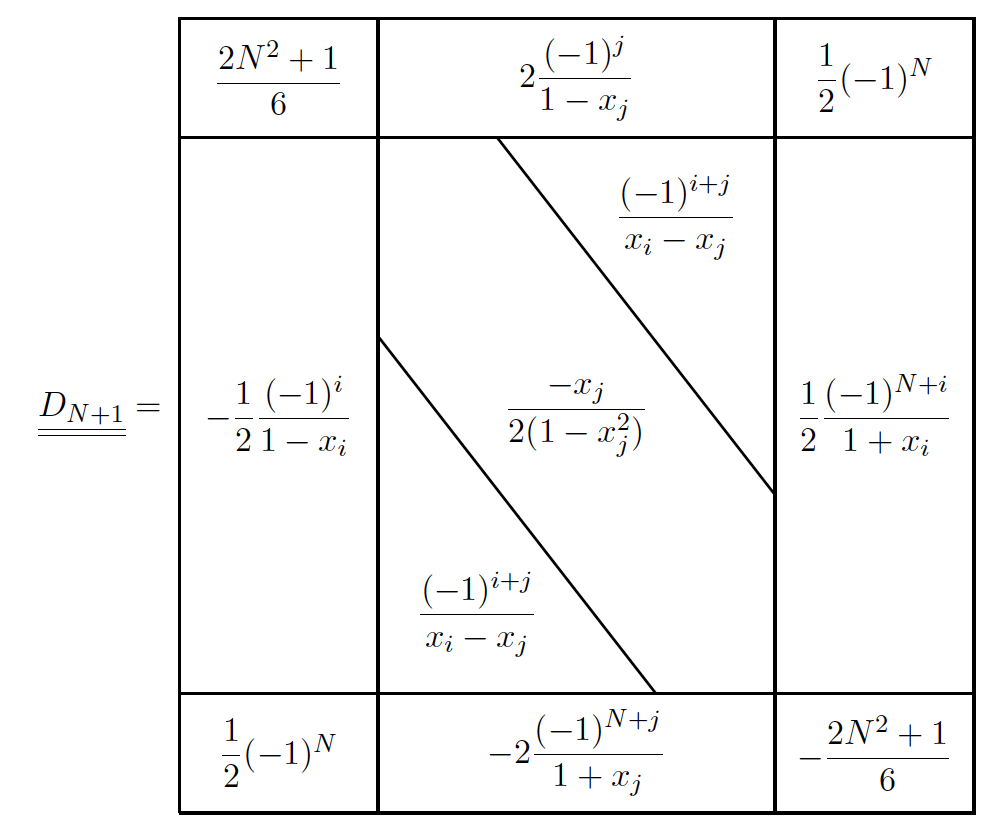
\includegraphics[scale=0.5]{figures/Chebyshev.jpg}
% 	\caption{This differentitation matrix works with chebyshev points.\cite{Peterson:2}\cite{Trefethen:7}}
% \end{figure}
\par
Thus, 
\begin{align}
    \vec{W_{p}}_{, t} + \lambda_{p} \, \vec{W_{p}}_{, s} = \sum_{q=1}^{M} F_{pq} \, \vec{W_{q}} \quad \rightarrow \quad
    \vec{W_{p}}_{, t} + \lambda_{p} \, \mat{D} \, \vec{W_{p}} = \sum_{q=1}^{M} F_{pq} \, \vec{W_{q}}
\end{align}
As usual, we need to also enforce boundary conditions (in particular, Dirichlet boundary conditions).
Since we are working a system of hyperbolic PDEs, we enforce inflow conditions:
\begin{itemize}
    \item If $\lambda_{p} > 0$, we enforce left inflow boundary conditions
    \item If $\lambda_{p} < 0$, we enforce right inflow boundary conditions
\end{itemize}
We can enforce the above inflow boundary conditions by modifying the appropriate columns and rows of $\mat{D}$ in the $p^{th}$ equation:
\begin{itemize}
    \item If $\lambda_{p} > 0$, we zero out the last column and last row of $\mat{D}$
    \item If $\lambda_{p} < 0$, we zero out the first column and first row of $\mat{D}$
\end{itemize}
\textbf{Note:} The above enforcement scheme makes sense in this context because the Chebyshev points of the second kind are ordered in \textit{decreasing} order from $1$ to $-1$.
\par 
Thus,
\begin{align}
    \vec{W_{p}}_{, t} + \lambda_{p} \, \mat{D} \, \vec{W_{p}} = \sum_{q=1}^{M} F_{pq} \, \vec{W_{q}} \quad \rightarrow \quad
    \vec{W_{p}}_{, t} + \lambda_{p} \, \mat{D_{p}} \, \vec{W_{p}} = \sum_{q=1}^{M} F_{pq} \, \vec{W_{q}}
\end{align}

\subsubsection{Temporal Discretization of the PDE}

Recall that we spatially discretized the $p^{th}$ equation in the above system to obtain
\begin{align}
    \vec{W_{p}}_{, t} + \lambda_{p} \, \mat{D_{p}} \, \vec{W_{p}} = \sum_{q=1}^{M} F_{pq} \, \vec{W_{q}}
\end{align}
We have not yet temporally discretized the system, but we have more freedom with picking time-stepping methods.
For this project, we adapted a \textbf{third-order}, \textbf{L-stable} IMEX Runge-Kutta scheme presented in \cite{PieracciniPuppo:3}.
The scheme is given as follows:
\begin{itemize}
    \item We have knowledge of the solution vectors $\vec{W_{p}}^{(n)}$ at some initial time-step $n$ for each equation $p = 1, 2, \hdots, M$
    \item In the first stage, we perform the following updates for equations $p = 1, 2, \hdots, M$:
    \begin{align}
        \vec{W_{p}}^{(1)} & = \vec{W_{p}}^{(n)} - \Delta t \, a_{11} \, \lambda_{p} \, \mat{D_{p}} \, \vec{W_{p}}^{(1)} \label{time_stepping:line_1}
    \end{align}
    \item For each stage $i = 2, \hdots, \nu$ (where $\nu = 4$ is the last stage), we perform the following updates for equations $p = 1, 2, \hdots, M$:
    \begin{align}
        \vec{W_{p}}^{(i)} & = \vec{W_{p}}^{(n)} + \Delta t \, \sum_{l=1}^{i-1} \widetilde{a}_{il} \sum_{q=1}^{M} F_{pq} \vec{W_{q}}^{(l)} - \Delta t \, \sum_{l=1}^{i} a_{il} \, \lambda_{p} \, \mat{D_{p}} \, \vec{W_{p}}^{(l)} \label{time_stepping:line_2}
    \end{align}
    \item To obtain the solution vectors $\vec{W_{p}}^{(n+1)}$ at the next time-step $(n+1)$, we perform the following updates for equations $p = 1, 2, \hdots, M$:
    \begin{align}
        \vec{W_{p}}^{(n+1)} & = \vec{W_{p}}^{(n)} + \Delta t \, \sum_{i=1}^{\nu} \widetilde{w}_{i} \sum_{q=1}^{M} F_{pq} \, \vec{W_{q}}^{(i)} - \Delta t \, \sum_{i=1}^{\nu} w_{i} \lambda_{p} \mat{D_{p}} \, \vec{W_{p}}^{(i)} \label{time_stepping:line_3}
    \end{align}
\end{itemize}
% \begin{align}
%   \vec{W_{p}}^{(1)} & = \vec{W_{p}}^{(n)} - \Delta t \, a_{11} \, \lambda_{p} \, \mat{D_{p}} \, \vec{W_{p}}^{(1)} \label{time_stepping:line_1} \\
%   \vec{W_{p}}^{(i)} & = \vec{W_{p}}^{(n)} + \Delta t \, \sum_{l=1}^{i-1} \widetilde{a}_{il} \sum_{q=1}^{M} F_{pq} \vec{W_{q}}^{(l)} - \Delta t \, \sum_{l=1}^{i} a_{il} \, \lambda_{p} \, \mat{D_{p}} \, \vec{W_{p}}^{(l)} \label{time_stepping:line_2} \\
%     \vec{W_{p}}^{(n+1)} & = \vec{W_{p}}^{(n)} + \Delta t \, \sum_{i=1}^{\nu} \widetilde{w}_{i} \sum_{q=1}^{M} F_{pq} \, \vec{W_{q}}^{(i)} - \Delta t \, \sum_{i=1}^{\nu} w_{i} \lambda_{p} \mat{D_{p}} \, \vec{W_{p}}^{(i)} \label{time_stepping:line_3}
% \end{align}
% In \ref{time_stepping:line_1}, we perform this update for $p = 1, 2, \hdots, M$.
% In \ref{time_stepping:line_2}, we perform this update first for every $i = 2, \hdots, \nu$ then for every $p = 1, 2, \hdots, M$, where $\nu = 4$ is the last stage number.
% In \ref{time_stepping:line_3}, we perform this update for $p = 1, 2, \hdots, M$.

\subsubsection{Solving the System via the Matrix Exponential}

We can also solve the above system using the matrix exponential.
Recall that the $p^{th}$ equation in the spatially discretized system is given by
\begin{align}
    \vec{W_{p}}_{, t} + \lambda_{p} \, \mat{D_{p}} \, \vec{W_{p}} = \sum_{q=1}^{M} F_{pq} \, \vec{W_{q}}
\end{align}
We can rearrange the above to obtain
\begin{align}
    \vec{W_{p}}_{, t} = -\lambda_{p} \, \mat{D_{p}} \, \vec{W_{p}} + \sum_{q=1}^{M} F_{pq} \, \vec{W_{q}}
\end{align}
We can then compute the solution of the entire system at the final time $t_{f}$ via the matrix exponential:
\begin{align*}
    \begin{bmatrix}
        \vec{W_{1}} \\
        \vec{W_{2}} \\
        \vdots \\
        \vec{W_{M}}
    \end{bmatrix}
    & = \exp \left(-t_{f}
    \begin{bmatrix}
    -\lambda_{1} \, \mat{D_{1}} + F_{11} \, \mat{I} & F_{12} \, \mat{I} & \hdots & F_{1m} \, \mat{I}  \\
    F_{21} \, \mat{I} & -\lambda_{2} \, \mat{D_{2}} + F_{22} \, \mat{I} & \hdots & F_{2m} \, \mat{I}  \\
    \vdots & \vdots & \ddots & \vdots \\
    F_{m1} \, \mat{I} & \hdots & F_{m(m-1)} \, \mat{I} & -\lambda_{m} \, \mat{D_{m}} + F_{mm} \, \mat{I}
    \end{bmatrix} \right)
    \vec{W_0}
\end{align*}
where
\begin{align}
    \vec{W_{0}} & =
    \begin{bmatrix}
        \vec{W_{1}}^{(0)} \\
        \vec{W_{2}}^{(0)} \\
        \vdots \\
        \vec{W_{m}}^{(0)}
    \end{bmatrix} \in \mathbb{R}^{(M \cdot N_{s})}
\end{align}
is a vector of discretized initial conditions corresponding to the $M$ equations in the system.  
% !TEX root = main.tex

\newpage
\section{Results}

%%%%%%%%%%%%%%%%%%%%%%%%%%%%%%%%%%%%%%%%%%%%%%%%%%%%%%%%%%%%%%%%%%
\subsection{Examples}

We first demonstrate a qualitative example of this approach applied to a 2D wave equation with a radially symmetric initial condition.
\FloatBarrier
%\begin{center}
\begin{figure}[H]
    \begin{tabular}{cc}
        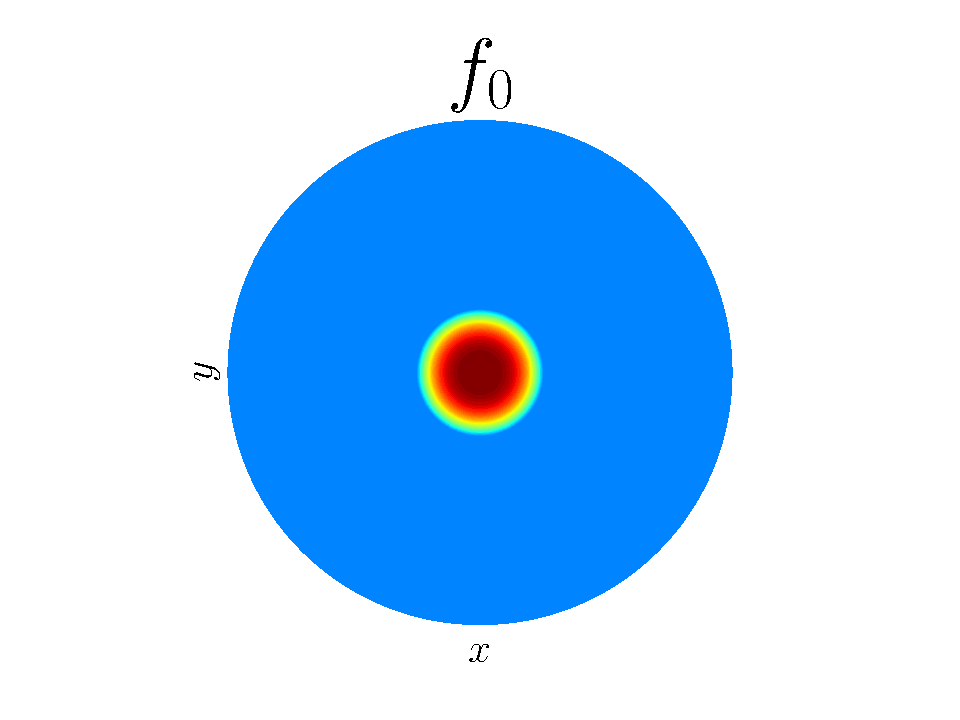
\includegraphics[height=5cm]{figures/Physical_Initial.pdf} & 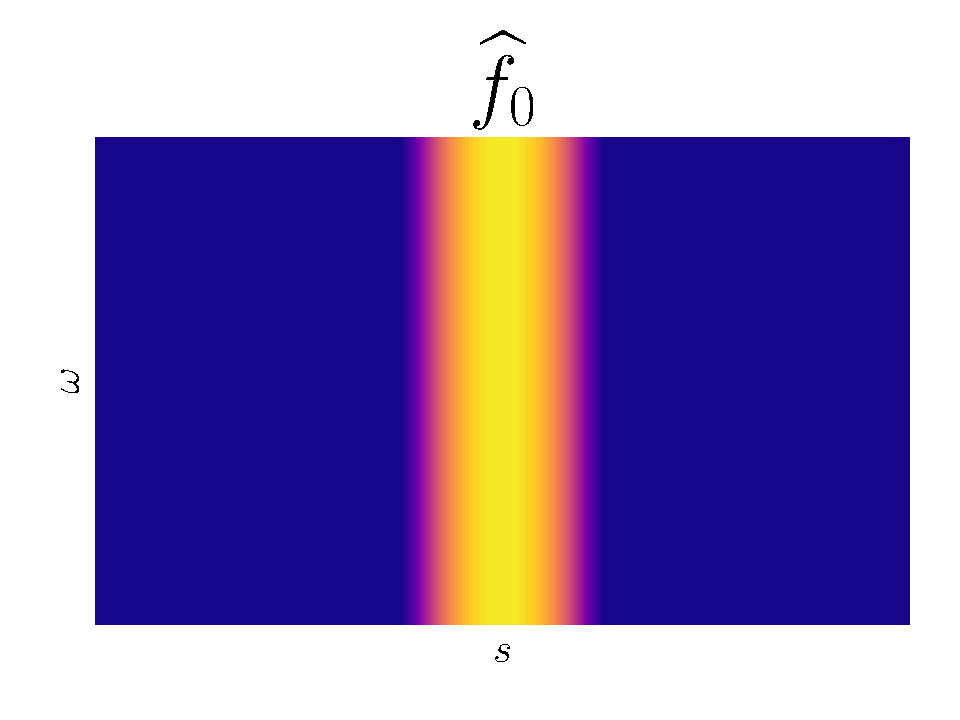
\includegraphics[height=5cm]{figures/Radon_Initial.pdf} \\ 
        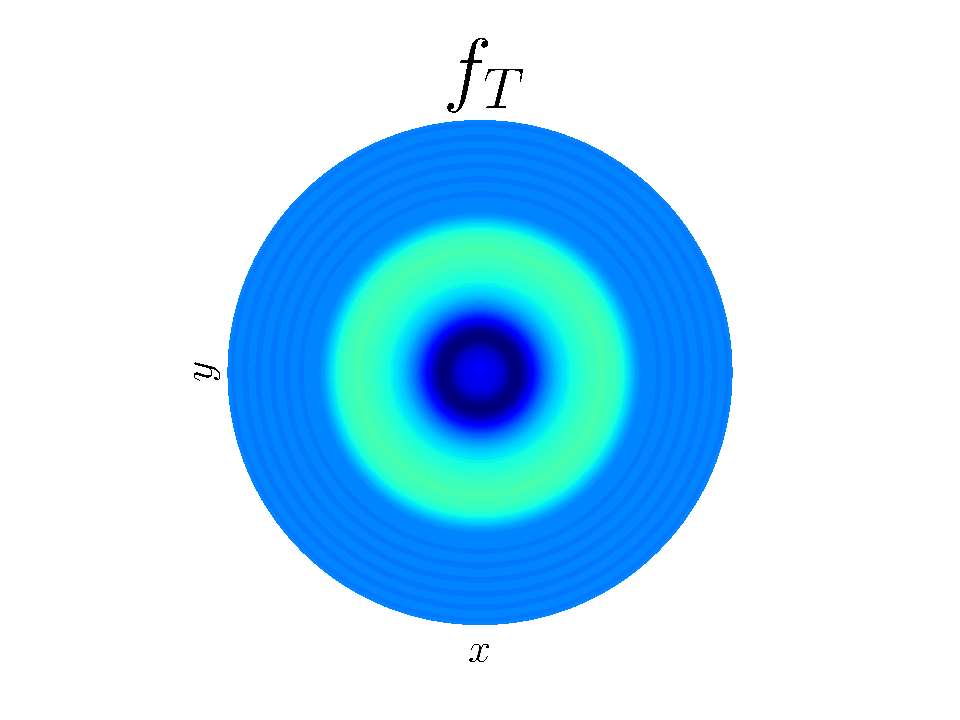
\includegraphics[height=5cm]{figures/Physical_Final.pdf} & 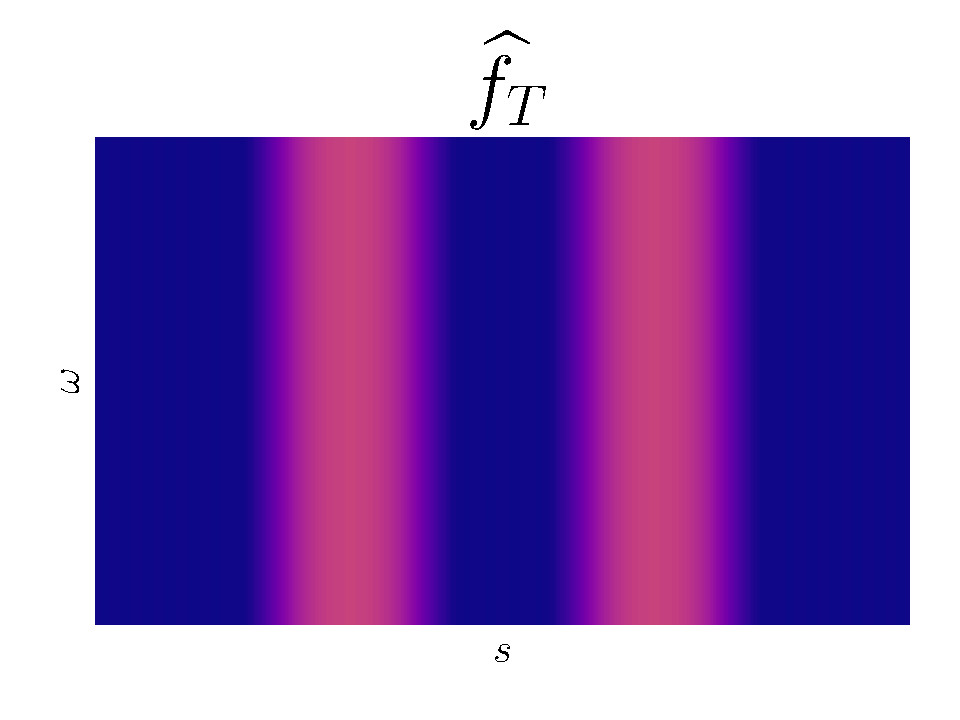
\includegraphics[height=5cm]{figures/Radon_Final.pdf}
    \end{tabular}
    \caption{Wave equation initial conditions (top) and final solution (bottom) \\ in physical (left) and Radon space (right)}
\end{figure}
%\end{center}
\FloatBarrier
In the above figures, we can observe the effect of Radial symmetry on our method. In particular, each sample of radon space is identical, as the transform is independent of the angle $\omega$. Moreover, the inversion process is much simpler, as the Radon transform matrix $\mat{R}$ is initially well conditioned and can be simply inverted.

\newpage
We can repeat this process for the radially symmetric $P_1$ equations. We use the standard initial condition, the following approximate to a Dirac delta function with $\alpha = 0.03$:
\begin{align*}
    q_0(x, y) = \frac{1}{4\pi\alpha^2}e^{\frac{ -(x^2 + y^2) }{4\alpha^2} }
\end{align*}
\FloatBarrier
\begin{center}
\begin{figure}[H]
    \begin{tabular}{c|c}
        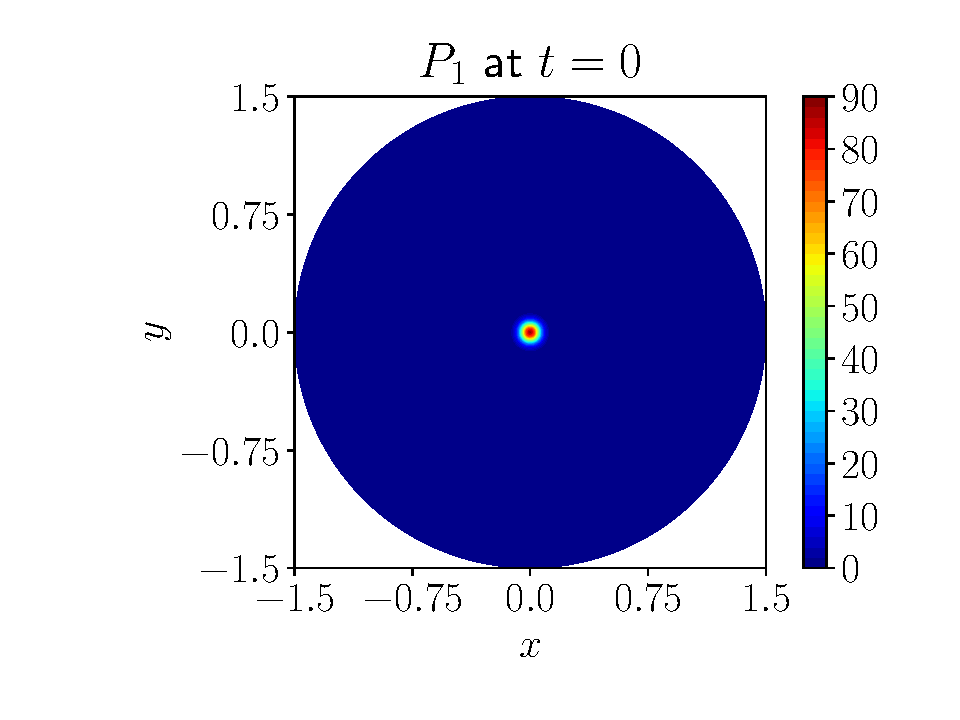
\includegraphics[height=5cm]{figures/physical_inital_p1.pdf} & 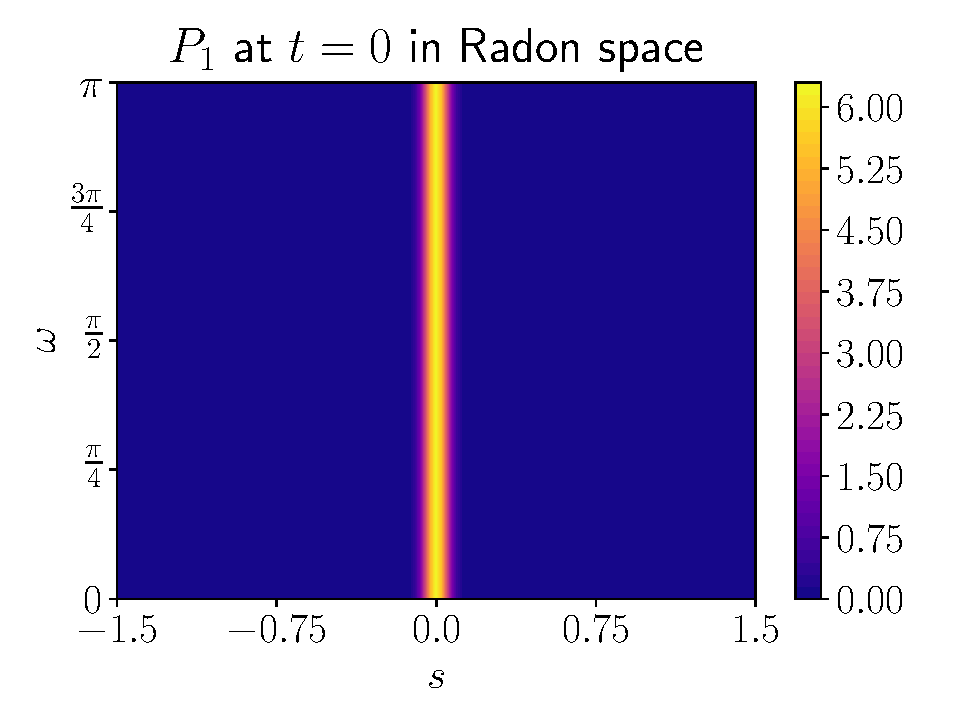
\includegraphics[height=5cm]{figures/radon_inital_p1.pdf} \\ \hline
        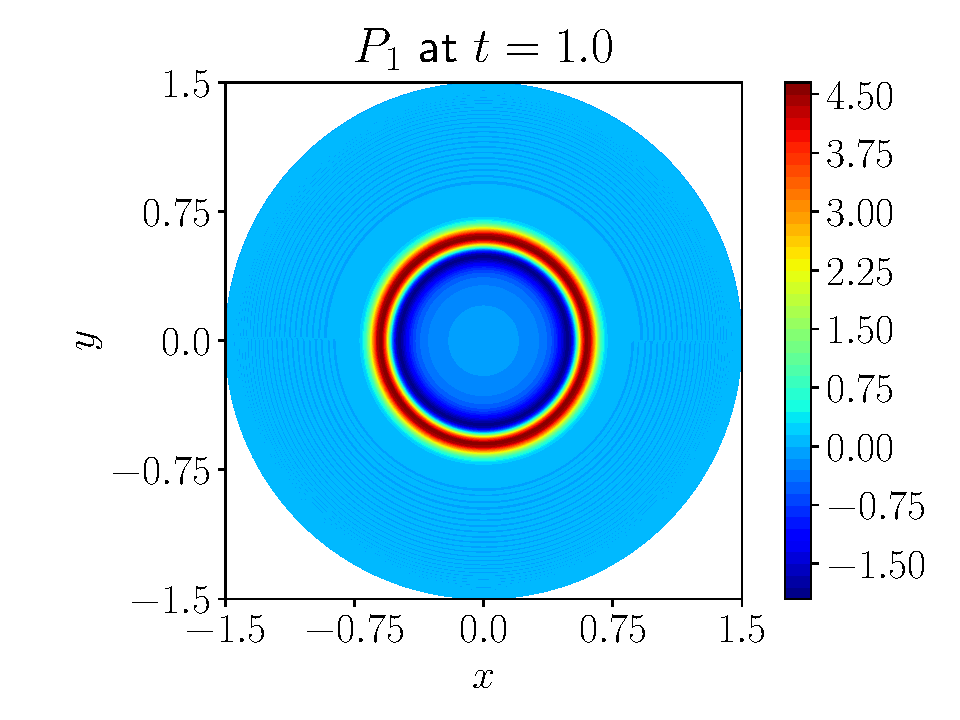
\includegraphics[height=5cm]{figures/physical_final_p1.pdf} & 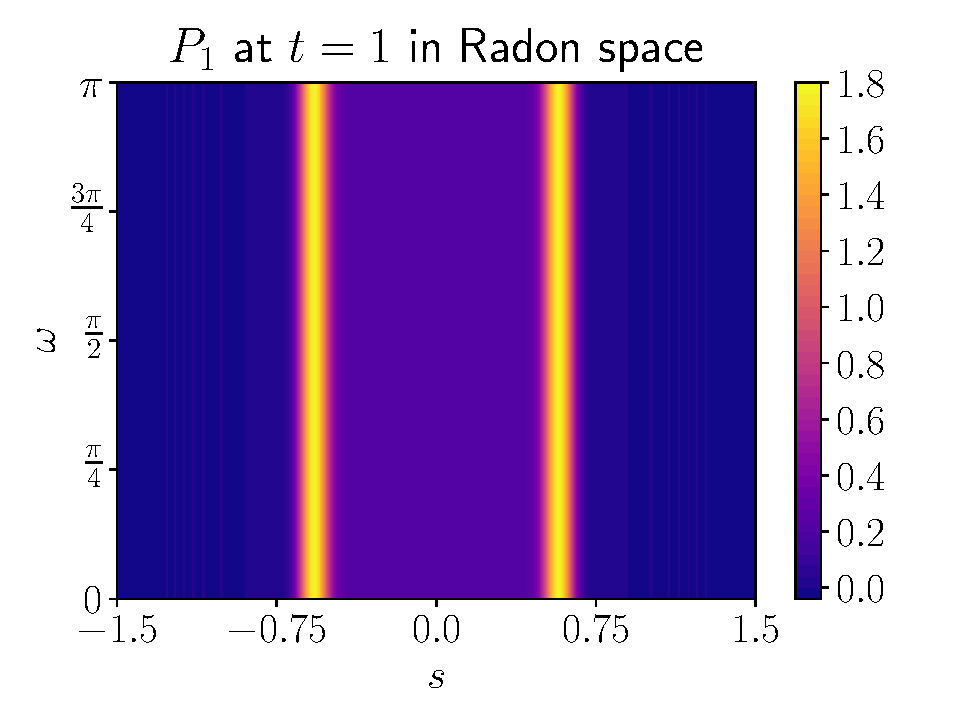
\includegraphics[height=5cm]{figures/radon_final_p1.pdf}
    \end{tabular}
    \caption{$P_1$ initial conditions (top) and final solution (bottom) \\ in physical (left) and Radon space (right)}
\end{figure}
\end{center}
\FloatBarrier
Because the $P_N$ equations themselves are only approximations of radiative transfer, we increase $N$ and compare our results to those in\cite{Shin:6}, as we see on the following page.

\newpage
\FloatBarrier
\begin{center}
\begin{tabular}{c|c}                    
    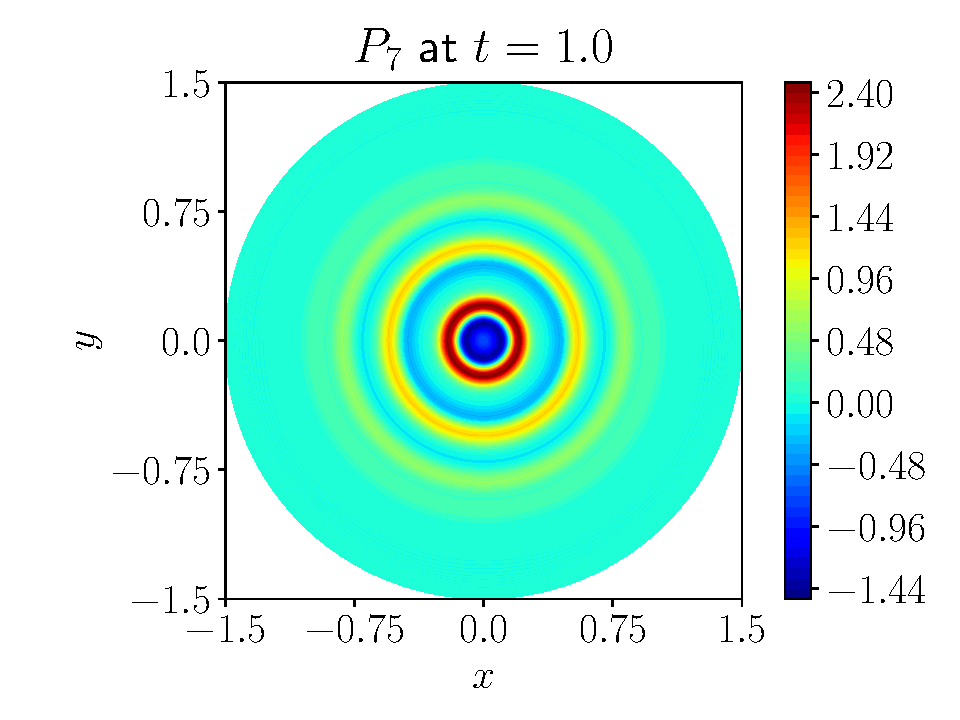
\includegraphics[height=0.4\linewidth]{figures/physical_final_p7.pdf} &
    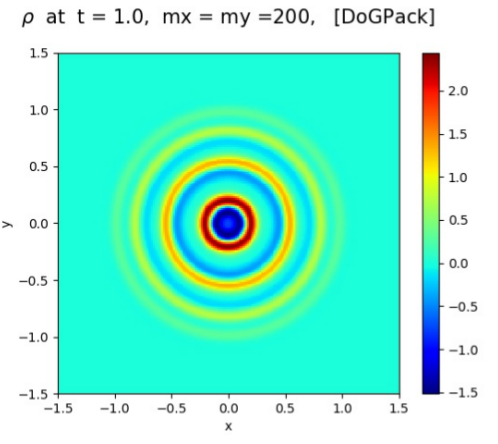
\includegraphics[height=0.4\linewidth]{figures/Minwoo_p7.png} \\
    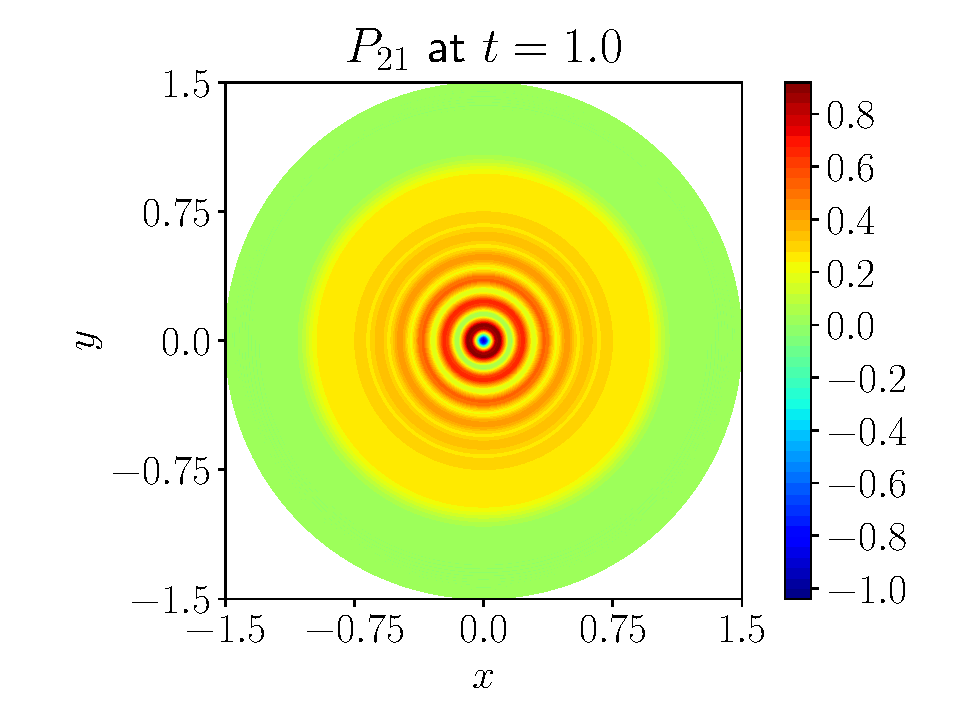
\includegraphics[height=0.4\linewidth]{figures/physical_final_p21.pdf} &
    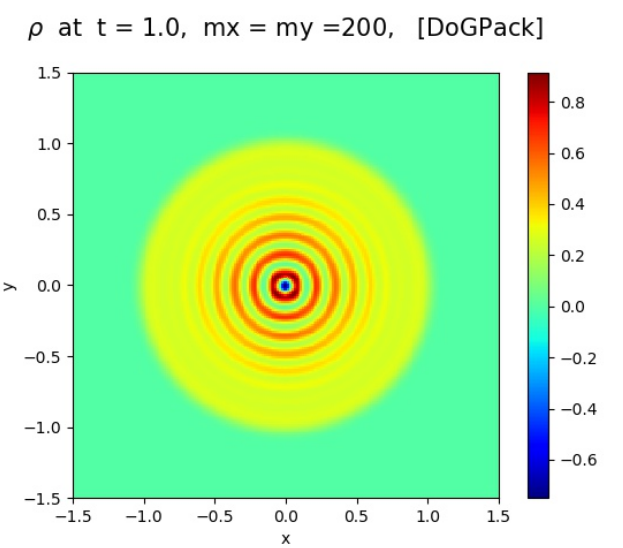
\includegraphics[height=0.4\linewidth]{figures/Minwoo_p21.png} \\
    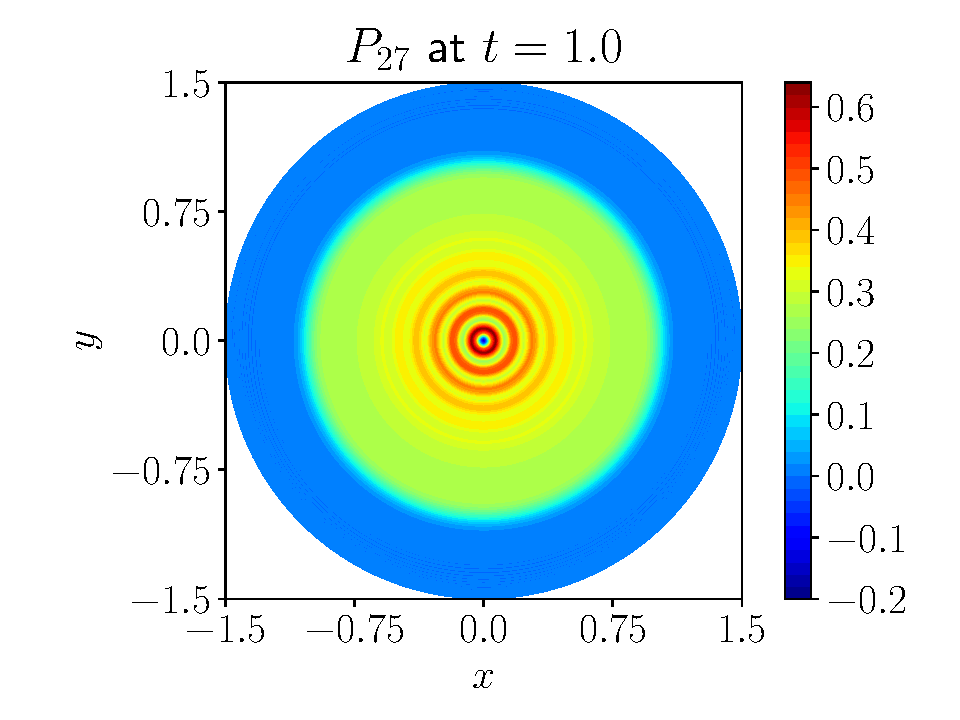
\includegraphics[height=0.4\linewidth]{figures/physical_final_p27.pdf} &
    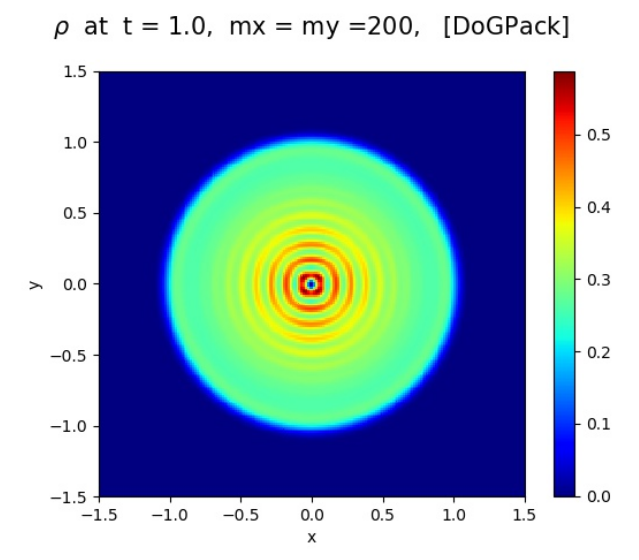
\includegraphics[height=0.4\linewidth]{figures/Minwoo_p27.png} \\
    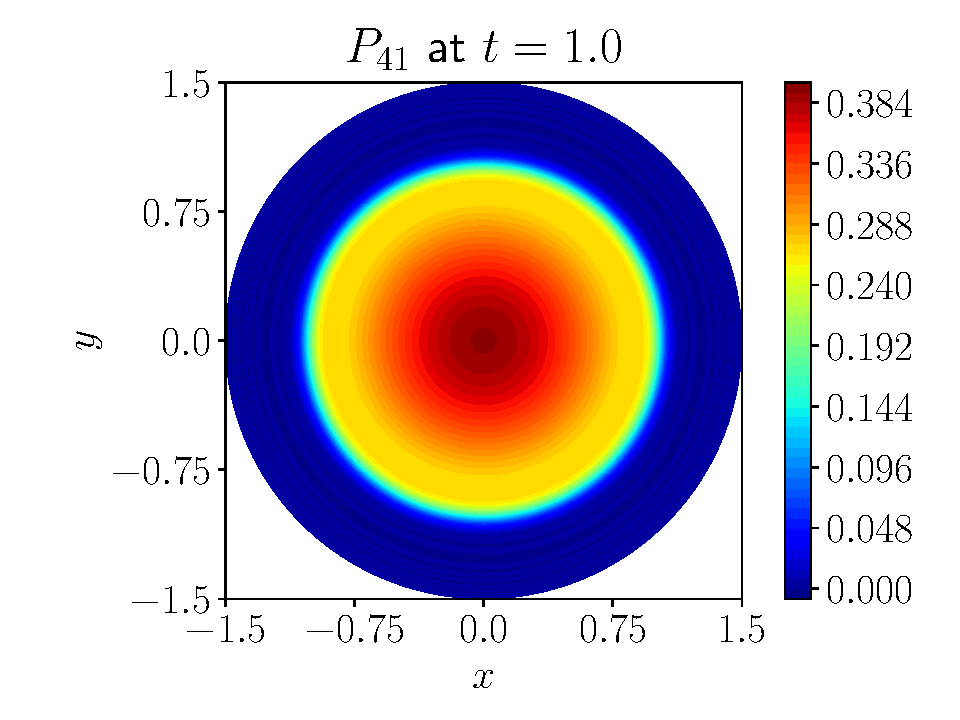
\includegraphics[height=0.4\linewidth]{figures/physical_final_p41.pdf} &
    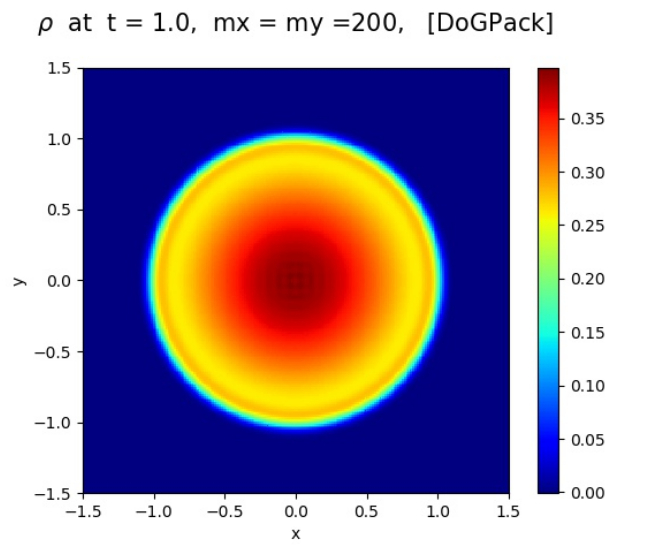
\includegraphics[height=0.4\linewidth]{figures/Minwoo_p41.png}
\end{tabular}
\end{center}    
%%%%%%%%%%%%%%%%%%%%%%%%%%%%%%%%%%%%%%%%%%%%%%%%%%%%%%%%%%%%%%%%%%
\subsection{Convergence}

In general, forming exact solutions to the $P_N$ equations is difficult.
In place of an exact solution, a high-resolution numerical solution to the radially symmetric $P_1$ equations is found with the following system of PDEs.
This formulation takes advantage of the radial symmetry to rewrite the system in polar coordinates, resulting in a 1D slice of the solution.
This PDE can be solved through any of the standard timestepping methods discussed above.
For their use as a comparison tool, this reference solution is interpolated across the 1D domain.
The solution in Radon space can then be obtained by performing a forward Radon transform of this physical solution.
\begin{align*}
	\begin{bmatrix}
		p \\
		u_{r}
	\end{bmatrix}_{, t} + 
	\begin{bmatrix}
		0 & \frac{1}{\sqrt{3}} \\
		\frac{1}{\sqrt{3}} & 0
	\end{bmatrix}
	\begin{bmatrix}
		p \\
		u_{r}
	\end{bmatrix}_{, r} = 
	\begin{bmatrix}
		-\frac{1}{\sqrt{3}} \frac{1}{r} u_{r} \\
		-\sigma u_{r}
	\end{bmatrix}
\end{align*}
To simplify the convergence studies, only a single slice of the solution obtained through the Radon method is compared.
When the $L_\infty$ norm is used, the error between the reference solution and the approximated solution is identical between any diameter of the mesh.
Thus the $L_\infty$ error across any single diameter is equal to that over the entire domain.
Additionally, radial symmetry indicates that the discretization in $\omega$ is arbitrary, and the following convergence test only takes into account the discretization across each diameter.
%\FloatBarrier
\begin{center}
    \begin{figure}[H]
        \begin{tabular}{cc}                    
            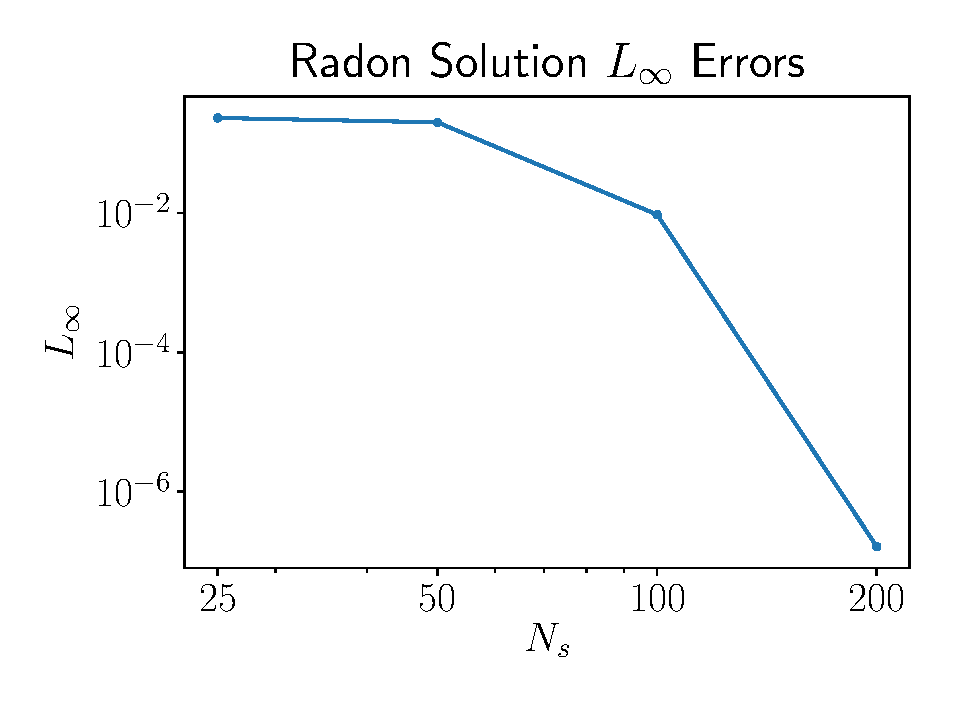
\includegraphics[height=0.35\linewidth]{figures/Convergence_Radon_Errors.pdf} &
            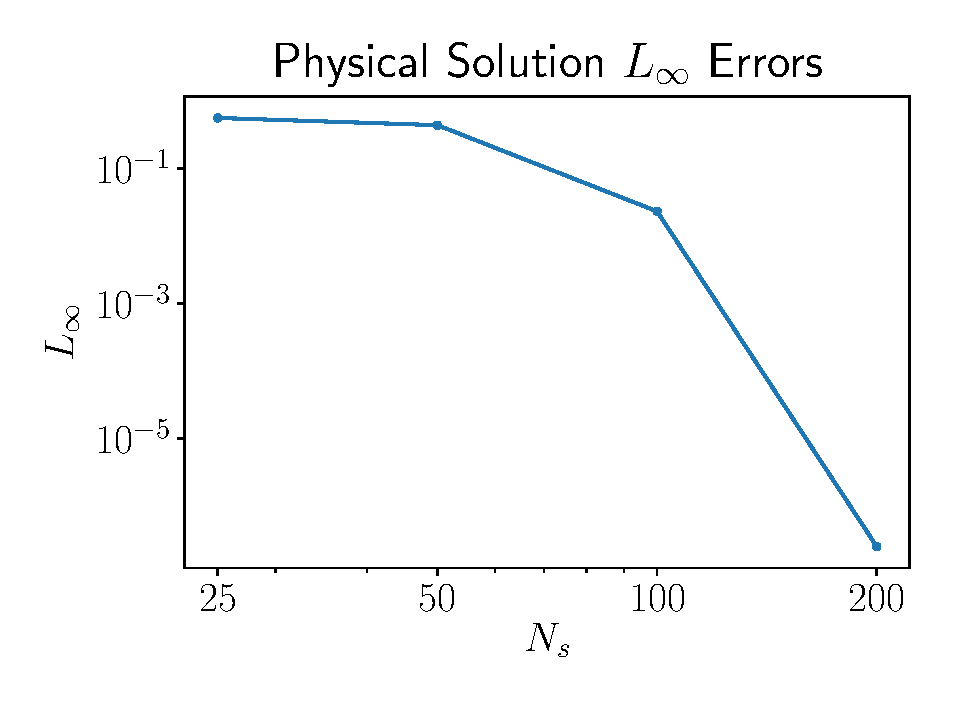
\includegraphics[height=0.35\linewidth]{figures/Convergence_Physical_Errors.pdf}
        \end{tabular}
    \captionof{figure}{$L_\infty$-Norm for radially symmetric initial conditions}
    \end{figure}
\end{center}
%\FloatBarrier
As expected, the convergence of the overall method is spectrally accurate in $N_s$.
This is because the only error present in the solution comes from insufficiently approximating the initial condition.
All other calculations, such as the interpolation, spectral differentiation, and quadrature, are all performed with spectral accuracy.

Computing convergence rates precisely is more difficult for non-radially symmetric problems, as there are no exact solutions to reference.
To counteract this, the same reference solution for the symmetric case is used, but shifted in the positive $x$ direction by some constant.
Then, the experimental $P_1$ solution can be found by translating the initial condition by the same amount, and considering the cross section across the $x$-axis.
While not a precise convergence study, one can still see that the solution approaches the true value.
For these problems, the effect of $N_s$ and $N_\omega$ must be considered independently of one another.

We begin by fixing $N_\omega = 200$, and varying $N_s$, as the timestepping is independent of the problem's symmetry.
That is to say, the solution in Radon space should be as accurate as the symmetric case.
%\FloatBarrier
\begin{center}
\begin{figure}[H]
\begin{tabular}{cc}                    
    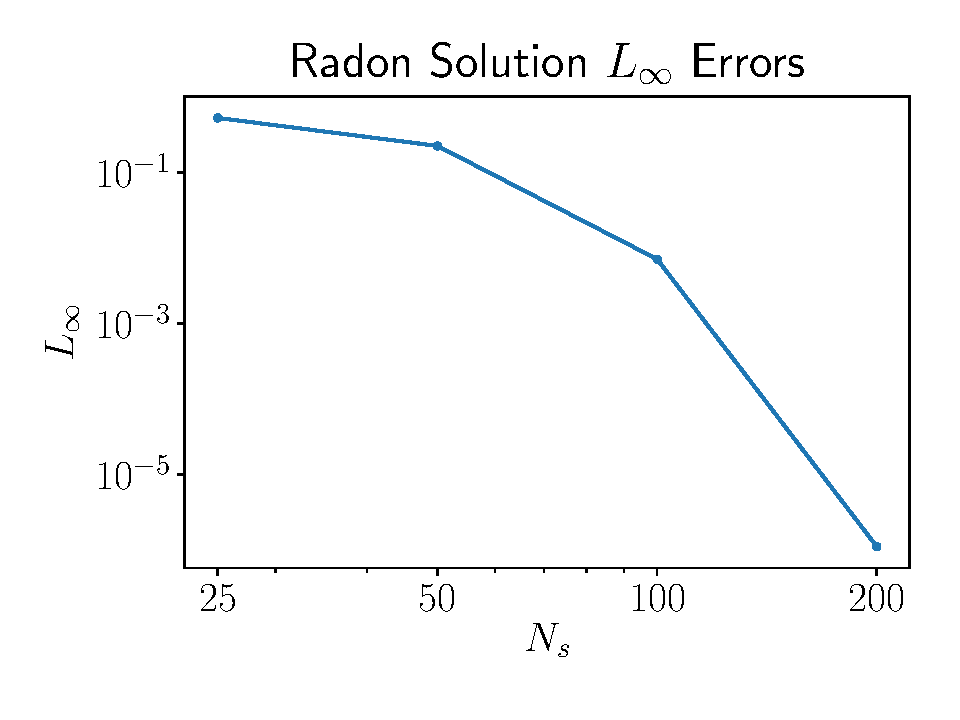
\includegraphics[height=0.35\linewidth]{figures/Convergence_Radon_Errors_Ns.pdf} &
    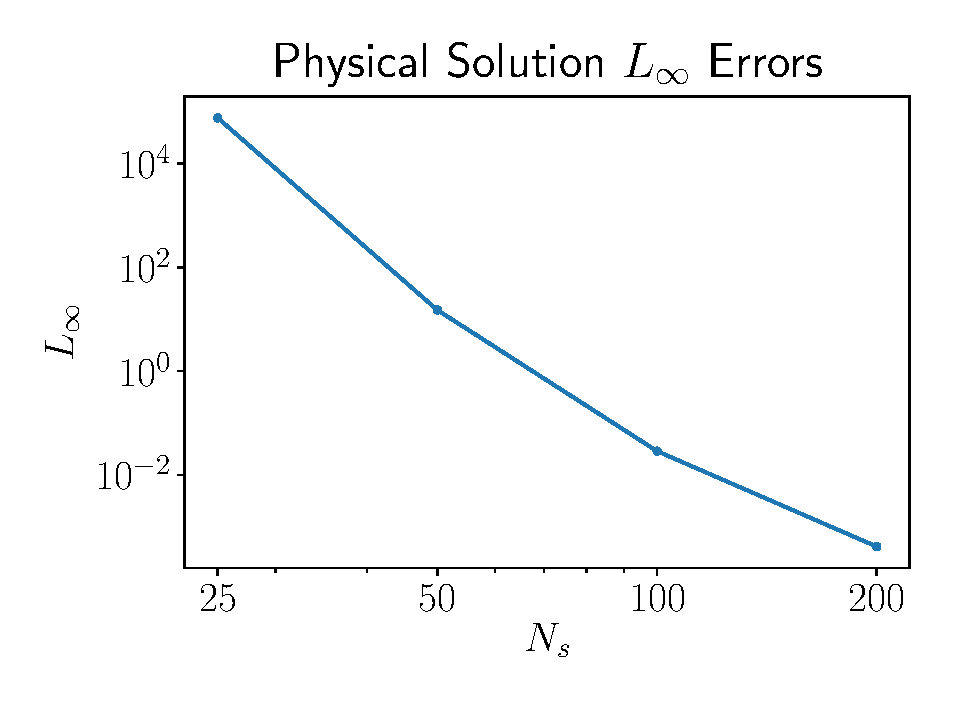
\includegraphics[height=0.35\linewidth]{figures/Convergence_Physical_Errors_Ns.pdf}
\end{tabular}
\captionof{figure}{$L_\infty$-Norm for radially symmetric initial conditions}
\end{figure}
\end{center}
%\FloatBarrier
As we see, this is the case.
We also observe that now the solution in physical space no longer has the same rate of accuracy, as the solution is limited by $N_\omega$.

We now perform the same test, but fixing $N_s$ and varying $N_\omega$.
Across each of these examples, the solution in Radon space is identical, as the timestepping is once again dependent only on the discretization along each diameter.
However, the solution in physical space is heavily dependent on the number of $N_\omega$.
We expect the solution to be fourth-order accurate, as this is the lowest convergence rate across all the component methods (owing to the radial interpolation across diameters).
%\FloatBarrier
\begin{center}
\begin{figure}[H]
	\centering
    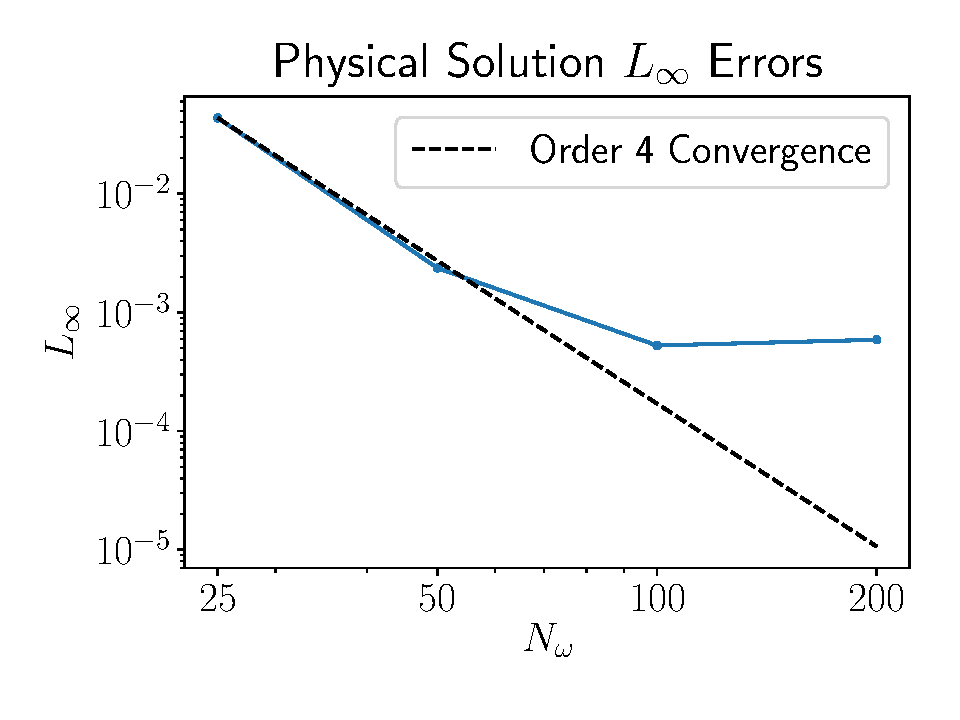
\includegraphics[height=0.35\linewidth]{figures/Convergence_Physical_Errors_Nw.pdf}
    \captionof{figure}{$L_\infty$-Norm for radially symmetric initial conditions}
\end{figure}
\end{center}
%\FloatBarrier
In practice however, we observe that while the error in the solution does decrease, it does not decrease quite as expected.
While the error is already relatively low even for low values of $N_\omega$, the desired convergence rate is only observed across the first two experiments.
Moreover the reasons for this are largely unknown at this time.
It is suspected that, rather than the method simply not being as accurate as hypothesized, there is some hidden source of error that is limiting the efficacy of the inverse Radon transform.
Possible sources of this error are a failure to accurately capture the initial condition with $N_s=200$ or a not sufficiently accurate timestepping method.
It is also possible that there is an issue with the reference solution, which is, again, only a high-resolution approximation of the true solution.
It is our hope that by addressing some or all of these issues, we can obtain results consistent with our overarching theory.
That being said, the potential payoffs of this method are great, and we hope that further investigation will illuminate this.
% !TEX root = main.tex

\section*{Summary}

To summarize the project, the RT was used to bring the $P_N$ equations\cite{BrunnerHolloway:1} into radon space to solve a family of one dimensional PDEs instead of a two or more-dimensional PDE in real space.
Then, transport and time-stepping\cite{PieracciniPuppo:3} was used to solve the hyperbolic PDEs.
Last, the IRT was used to take the solution from radon space back to physical space.
% !TEX root = main.tex

\section*{Future Work}

For future work, there are a couple of routes that we would suggest.
First, adding spatially dependent collision terms to the $P_N$ equations.
The scope of this project did not cover those terms and assumed that any collision term was zero.
Next, a more sophisticated or higher order time-stepping scheme could be used to reduce any error that may have been encountered.
Finally, parallelization could be used to speed up the code that was written.
This could be accomplished by parallelizing the RT as well as parallelizing the separate angles.
% !TEX root = main.tex

\section*{Acknowledgments}

We would like to acknowledge the people and organizations that supported us through this research.
These people and organizations include: the NSF and the grant (DMS-1457443) that allowed us to travel to Iowa State University (ISU); ISU for hosting us for our time in Iowa; and most of all, to Dr. Rossmanith, our faculty mentor, and Christine Wiersma, our graduate student mentor, who were crucial to the completion of this research. 

\bibliographystyle{te}

\bibliography{bib}

\end{document}